% =====================================================================
%  Say, Echo, Do: Strategic Speech, Media Echo, and False Alarms
%  Conference version -- two-column, AAAS/Science palette
% =====================================================================
\documentclass[10pt,twocolumn,letterpaper]{article}

% ---------- Fonts & layout ------------------------------------------
\usepackage[T1]{fontenc}
\usepackage{mathptmx}
\usepackage[scaled=0.92]{helvet}
\usepackage[letterpaper,margin=0.75in,columnsep=0.28in]{geometry}
\usepackage{amsmath,amssymb,amsthm,mathtools,bm}
\usepackage{booktabs,tabularx,array,multirow}
\usepackage{enumitem}
\usepackage{xcolor}
\usepackage{tikz}
\usetikzlibrary{positioning,arrows.meta,calc,decorations.markings,decorations.pathreplacing,shapes.geometric}
\usepackage{pgfplots}
\pgfplotsset{compat=1.16}
\usepgfplotslibrary{groupplots,fillbetween}
\usepackage[most]{tcolorbox}
\usepackage{titlesec}
\usepackage[font=small,labelfont={sf,bf}]{caption}
\usepackage[numbers,sort&compress]{natbib}
\usepackage{microtype}
\usepackage[colorlinks=true,linkcolor=sNavy,citecolor=sNavy,urlcolor=sNavy]{hyperref}
\usepackage[capitalise,noabbrev,nameinlink]{cleveref}

\setlength{\parskip}{0pt}
\setlist{itemsep=1pt,topsep=2pt,parsep=0pt,leftmargin=*}

% ---------- AAAS (Science) palette ----------------------------------
\definecolor{ink}{HTML}{1B1919}
\definecolor{sNavy}{HTML}{3B4992}
\definecolor{sRed}{HTML}{EE0000}
\definecolor{sGreen}{HTML}{008B45}
\definecolor{sPurple}{HTML}{631879}
\definecolor{sTeal}{HTML}{008280}
\definecolor{sCrimson}{HTML}{BB0021}
\definecolor{sViolet}{HTML}{5F559B}
\definecolor{sMagenta}{HTML}{A20056}
\definecolor{sGray}{HTML}{808180}
\colorlet{say}{sPurple}
\colorlet{echo}{sCrimson}
\colorlet{do}{sNavy}
\colorlet{good}{sGreen}

% ---------- Headings & captions ---------------------------------------
\titleformat{\section}{\sffamily\bfseries\large\color{ink}}{\thesection}{0.6em}{}
\titleformat{\subsection}{\sffamily\bfseries\normalsize\color{ink}}{\thesubsection}{0.5em}{}
\titleformat{\paragraph}[runin]{\sffamily\bfseries\small}{}{}{}[.]
\titlespacing*{\section}{0pt}{10pt}{4pt}
\titlespacing*{\subsection}{0pt}{7pt}{3pt}
\titlespacing*{\paragraph}{0pt}{4pt}{0.6em}
\DeclareCaptionLabelSeparator{pipe}{\hspace{0.45em}\textbar\hspace{0.45em}}
\captionsetup{labelsep=pipe,figurename=Fig.,tablename=Table,skip=4pt}
\setlength{\textfloatsep}{10pt plus 2pt minus 2pt}
\setlength{\dbltextfloatsep}{10pt plus 2pt minus 2pt}

% ---------- Figure style ----------------------------------------------
\pgfplotsset{sci/.style={
  axis lines*=left,
  axis line style={ink!75, line width=0.5pt},
  tick style={ink!75, line width=0.4pt},
  tick align=outside, major tick length=2pt,
  tick label style={font=\sffamily\scriptsize, text=ink!85},
  label style={font=\sffamily\scriptsize, text=ink},
  legend style={font=\sffamily\scriptsize, draw=none, fill=none, row sep=-1pt},
  legend cell align=left,
  every axis plot/.append style={line width=1.0pt},
  xticklabel={\pgfmathprintnumber[assume math mode=true]{\tick}},
  yticklabel={\pgfmathprintnumber[assume math mode=true]{\tick}},
}}
\tikzset{
  numb/.style={circle, draw=ink, fill=white, line width=0.5pt, inner sep=0.6pt, font=\sffamily\bfseries\tiny, text=ink},
  lbl/.style={font=\sffamily\scriptsize, text=ink},
}
\newcommand{\panel}[1]{\par\noindent{\sffamily\bfseries\normalsize #1}\par\vspace{-9pt}}

% ---------- Theorems ---------------------------------------------------
\theoremstyle{plain}
\newtheorem{theorem}{Theorem}
\newtheorem{proposition}[theorem]{Proposition}
\newtheorem{lemma}[theorem]{Lemma}
\newtheorem{corollary}[theorem]{Corollary}
\theoremstyle{definition}
\newtheorem{assumption}{Assumption}
\newtheorem{definition}[theorem]{Definition}
\theoremstyle{remark}
\newtheorem{remark}[theorem]{Remark}
\crefname{assumption}{Assumption}{Assumptions}
\crefname{remark}{Remark}{Remarks}

\newtcolorbox{takeaway}[1]{enhanced,breakable,colback=sNavy!5,colframe=sNavy!5,
  borderline west={2pt}{0pt}{sNavy},arc=0pt,outer arc=0pt,left=6pt,right=5pt,top=3pt,bottom=3pt,
  fontupper=\small,before upper={\textsf{\textbf{\color{sNavy}#1}}\enspace}}

% ---------- Macros -----------------------------------------------------
\newcommand{\R}{\mathbb{R}}
\newcommand{\E}{\mathbb{E}}
\newcommand{\Prob}{\mathbb{P}}
\newcommand{\N}{\mathcal{N}}
\newcommand{\F}{\mathcal{F}}
\newcommand{\z}{\bm{z}}
\newcommand{\w}{\bm{w}}
\newcommand{\y}{\bm{y}}
\newcommand{\h}{\bm{h}}
\newcommand{\bphi}{\bm{\varphi}}
\newcommand{\ind}{\mathbf{1}}
\DeclareMathOperator{\sgn}{sgn}
\DeclareMathOperator{\Var}{Var}
\DeclareMathOperator{\Cov}{Cov}
\DeclareMathOperator{\KL}{KL}
\newcommand{\SAY}{\textcolor{say}{\textsf{\textbf{Say}}}}
\newcommand{\ECHO}{\textcolor{echo}{\textsf{\textbf{Echo}}}}
\newcommand{\DO}{\textcolor{do}{\textsf{\textbf{Do}}}}

% =====================================================================
\begin{document}

\twocolumn[{%
\begin{center}
{\sffamily\bfseries\LARGE \textcolor{say}{Say}, \textcolor{echo}{Echo}, \textcolor{do}{Do}:\par}
\vspace{3pt}
{\sffamily\bfseries\Large Strategic Speech, Media Echo, and the Economics of False Alarms\par}
\vspace{8pt}
{\sffamily\normalsize [Author Name]\textsuperscript{1}\par}
{\sffamily\footnotesize \textsuperscript{1}[Affiliation] \quad\textbullet\quad [email]\par}
\vspace{8pt}
\end{center}
\begin{center}
\begin{minipage}{0.88\textwidth}
\sffamily\small
\textbf{Abstract.} Markets hear three voices: what institutions \emph{say}, what the media \emph{echoes}, and what capital \emph{does}. We develop a theory of the disagreement between them. Our central result explains \emph{false alarms} endogenously. An institution that trades while addressing a partly credulous crowd optimally talks an asset down while buying it exactly when $\varphi^2<2\lambda k<\varphi$, where $\varphi$ is crowd credulity, $\lambda$ price impact and $k$ the cost of misreporting. It exaggerates and sells when $\varphi>1$. A distribution-free identity, $\Cov(r,\mathrm{Say})=\lambda\Cov(\mathrm{Do},\mathrm{Say})-\varphi\sigma_\varepsilon^2$, makes the observable covariance between words and deeds the switch that decides whether words should be followed or faded. Media virality, measured by the Hawkes branching ratio, yields a manipulation dichotomy: echo breeds false alarms in deep markets and exaggeration in shallow ones. When trust is learned adaptively, it converges to truth only if $\lambda k>1$; a flip bifurcation at $\lambda k=1$ creates a closed-form credibility cycle, stable for $\tfrac56<\lambda k<1$, that leads by period-doubling to chaos. For measurement, we prove an exact \emph{semantic declustering} theorem that separates news from echo using timing and embedding similarity. We show that return-aligned contrastive embeddings are affine isometries of market-outcome space, with a Pinsker certificate for imperfect training. We also show that L\'evy area identifies whether money moved before the narrative. Monte Carlo simulation confirms every closed form.
\end{minipage}
\end{center}
\vspace{10pt}
}]

% =====================================================================
\section{Introduction}\label{sec:intro}

A respected bank publishes a gloomy call. Headlines multiply. The stock falls, though by less than the noise suggests, and weeks later it trades higher. In hindsight, someone was buying all along (\cref{fig:teaser}a). Practitioners call such episodes \emph{false alarms}. Proving intent is neither possible nor necessary. What is possible is to measure the disagreement between three observable voices: \SAY\ (institutional statements such as ratings, notes and management tone), \ECHO\ (media repetition and amplification) and \DO\ (revealed allocation: holdings, insider trades, options flow and price).

We develop a theory of that disagreement and of how to trade it. Two principles organise the paper. \emph{Deeds over words}: when \SAY\ and \DO\ disagree, the optimal forecast is proportional to their weighted gap, and the \emph{sign} of their covariance decides whether words are followed or faded. \emph{Fade the echo, follow the news}: repetition carries no information, so its price effect must unwind, whereas under-weighted news drifts. The theory never prescribes blind contrarianism; it identifies which cell of \cref{fig:teaser}b applies.

\paragraph{Contributions} The results we believe to be new are:
\begin{itemize}
  \item \textbf{Endogenous false alarms} (\cref{sec:strategic}). A closed-form theory of optimal speech while trading, with a four-regime taxonomy: truth, shading, false alarm, and exaggeration with distribution (\cref{thm:speech,cor:taxonomy}).
  \item \textbf{The Say--Do covariance identity} (\cref{thm:identity}), which holds for any distribution and turns an observable statistic into a follow-or-fade switch.
  \item \textbf{A manipulation dichotomy under virality} (\cref{prop:virality}) and \textbf{credibility cycles} under adaptive trust (\cref{thm:cycles}), with explicit bifurcation thresholds $\lambda k=1$ and $\lambda k=\tfrac56$.
  \item \textbf{Semantic declustering} (\cref{thm:semantic}): exact, factorised news-versus-echo posteriors that combine timing with embedding similarity.
  \item \textbf{Embedding geometry with a certificate} (\cref{thm:racl,thm:robustnn}), \textbf{absorption as an interpretation gap} (\cref{thm:absorption}), and \textbf{lead--lag via L\'evy area} (\cref{thm:levy}).
\end{itemize}
The Gaussian follow-or-fade and Say--Do gap results (\cref{thm:followfade,thm:saydo}) are clean multi-channel statements of Bayesian updating. Regime detection, conformal calibration and Kelly sizing (\cref{app:extra}) are classical tools, included so that the paper is self-contained. Proofs are in \cref{app:proofs}.

\begin{figure*}[t]
\centering
\begin{minipage}[t]{0.37\textwidth}
\panel{a}
\centering
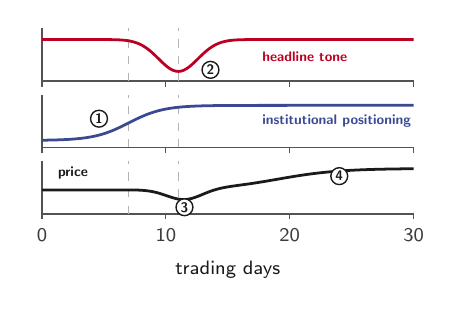
\begin{tikzpicture}
\begin{groupplot}[sci,
  group style={group size=1 by 3, vertical sep=5pt, xticklabels at=edge bottom},
  width=6.3cm, height=2.25cm, xmin=0, xmax=30, ytick=\empty,
  xtick={0,10,20,30}, no markers, samples=140, domain=0:30,
  ylabel style={align=center, font=\sffamily\scriptsize}, clip=false]
\nextgroupplot[ymin=-1.3, ymax=0.35]
  \addplot[sGray!60, thin, dashed, forget plot] coordinates {(7,-1.3) (7,0.35)};
  \addplot[sGray!60, thin, dashed, forget plot] coordinates {(11,-1.3) (11,0.35)};
  \addplot[echo] {-exp(-((x-11)^2)/5)};
  \node[lbl, text=echo, anchor=west, font=\sffamily\tiny\bfseries] at (axis cs:17,-0.55) {headline tone};
  \node[numb] at (axis cs:13.6,-0.95) {2};
\nextgroupplot[ymin=-0.2, ymax=1.3]
  \addplot[sGray!60, thin, dashed, forget plot] coordinates {(7,-0.2) (7,1.3)};
  \addplot[sGray!60, thin, dashed, forget plot] coordinates {(11,-0.2) (11,1.3)};
  \addplot[do] {1/(1+exp(-(x-7)/1.4))};
  \node[lbl, text=do, anchor=west, font=\sffamily\tiny\bfseries] at (axis cs:17,0.55) {institutional positioning};
  \node[numb] at (axis cs:4.6,0.62) {1};
\nextgroupplot[ymin=95, ymax=106, xlabel={trading days}]
  \addplot[sGray!60, thin, dashed, forget plot] coordinates {(7,95) (7,106)};
  \addplot[sGray!60, thin, dashed, forget plot] coordinates {(11,95) (11,106)};
  \addplot[ink] {100 - 2.2*exp(-((x-11.5)^2)/4) + 4.5/(1+exp(-(x-19)/2.5))};
  \node[numb] at (axis cs:11.5,96.4) {3};
  \node[numb] at (axis cs:24,102.9) {4};
  \node[lbl, text=ink, anchor=west, font=\sffamily\tiny\bfseries] at (axis cs:0.5,103.5) {price};
\end{groupplot}
\end{tikzpicture}
\end{minipage}\hfill
\begin{minipage}[t]{0.3\textwidth}
\panel{b}
\centering
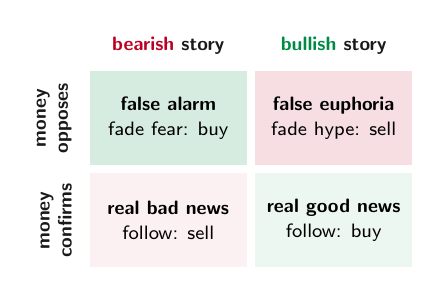
\begin{tikzpicture}[
  cell/.style={draw=white, line width=1.6pt, minimum width=2.05cm, minimum height=1.25cm, align=center, font=\sffamily\scriptsize},
  head/.style={font=\sffamily\scriptsize\bfseries, align=center, text=ink}]
\node[cell, fill=good!16] (a) at (0,0) {\textbf{false alarm}\\[1pt] fade fear: buy};
\node[cell, fill=echo!13] (b) at (2.1,0) {\textbf{false euphoria}\\[1pt] fade hype: sell};
\node[cell, fill=echo!6] (c) at (0,-1.3) {\textbf{real bad news}\\[1pt] follow: sell};
\node[cell, fill=good!7] (d) at (2.1,-1.3) {\textbf{real good news}\\[1pt] follow: buy};
\node[head, above=1pt of a] {\textcolor{echo}{bearish} story};
\node[head, above=1pt of b] {\textcolor{good}{bullish} story};
\node[head, rotate=90, anchor=south, align=center] at ($(a.west)+(-0.05,0)$) {money\\opposes};
\node[head, rotate=90, anchor=south, align=center] at ($(c.west)+(-0.05,0)$) {money\\confirms};
\end{tikzpicture}
\end{minipage}\hfill
\begin{minipage}[t]{0.3\textwidth}
\panel{c}
\centering
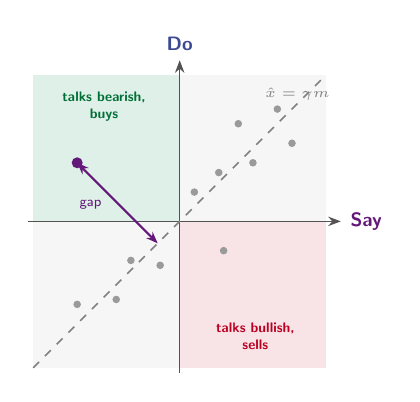
\begin{tikzpicture}[scale=0.62]
\fill[good!13] (-3,0) rectangle (0,3);
\fill[echo!11] (0,-3) rectangle (3,0);
\fill[ink!4] (0,0) rectangle (3,3);
\fill[ink!4] (-3,-3) rectangle (0,0);
\draw[-{Stealth[length=1.6mm]}, ink!75, line width=0.5pt] (-3.1,0) -- (3.3,0) node[right, lbl] {\SAY};
\draw[-{Stealth[length=1.6mm]}, ink!75, line width=0.5pt] (0,-3.1) -- (0,3.3) node[above, lbl] {\DO};
\draw[dashed, sGray, line width=0.6pt] (-3,-3) -- (3,3);
\node[lbl, text=sGray, anchor=west, font=\sffamily\tiny] at (1.55,2.6) {$\hat x=\gamma m$};
\node[lbl, text=good!80!black, align=center, font=\sffamily\tiny\bfseries] at (-1.55,2.35) {talks bearish,\\ buys};
\node[lbl, text=echo, align=center, font=\sffamily\tiny\bfseries] at (1.55,-2.35) {talks bullish,\\ sells};
\foreach \p in {(0.8,1.0),(1.5,1.2),(2.0,2.3),(-1.0,-0.8),(-2.1,-1.7),(0.3,0.6),(-1.3,-1.6),(2.3,1.6),(0.9,-0.6),(-0.4,-0.9),(1.2,2.0)}
  \fill[sGray!80] \p circle (2.2pt);
\fill[say] (-2.1,1.2) circle (3.2pt);
\draw[{Stealth[length=1.5mm]}-{Stealth[length=1.5mm]}, say, line width=0.8pt] (-2.1,1.2) -- (-0.45,-0.45);
\node[lbl, text=say, anchor=east, font=\sffamily\tiny] at (-1.4,0.35) {gap};
\end{tikzpicture}
\end{minipage}
\caption{\textbf{Three voices, one decision.} \textbf{a},~The false-alarm pattern (stylised): positioning builds (1) before the alarm (2); price falls far less than the alarm implies (3), then recovers (4). \textbf{b},~The narrative never decides the trade on its own; its agreement with money and price does. \textbf{c},~The Say--Do plane. The optimal forecast decreases with signed distance from the line $\hat x=\gamma m$ (\cref{thm:saydo}); the top-left quadrant is the false-alarm zone.}
\label{fig:teaser}
\end{figure*}

% =====================================================================
\section{Related Work}\label{sec:related}

\paragraph{Sentiment and returns} Media pessimism predicts price pressure followed by reversal \citep{tetlock2007}. Financial text needs domain-specific measurement \citep{loughran2011}, sentiment matters most where arbitrage is hard \citep{baker2006,shleifer1997,delong1990}, and attention drives demand \citep{barber2008,da2011}. Prices drift after headlines and reverse after no-news moves \citep{chan2003}, heterogeneous agents reconcile under- and overreaction \citep{hong1999}, and the same news is read differently across states \citep{veronesi1999}. Text factors and language models predict returns \citep{ke2019,araci2019,lopezlira2023}, subject to look-ahead bias \citep{glasserman2023}.

\paragraph{Informed trading and communication} Order flow reveals private information \citep{kyle1985,glosten1985}. Volume--return dynamics separate informed from hedging trades \citep{llorente2002}, predatory traders exploit predictable flow \citep{brunnermeier2005}, short sellers process news better \citep{engelberg2012}, insider trades split into informative and routine \citep{cohen2012}, and promotional articles move prices \citep{kogan2023}. Cheap talk \citep{crawford1982}, costly talk with credulous receivers \citep{kartik2007}, manipulation by informed ``gurus'' \citep{benabou1992} and rumour-based trading \citep{vanbommel2003} study how informed agents shape beliefs.

\paragraph{Mathematical tools} We use Hawkes processes \citep{hawkes1971} and their cluster representation \citep{hawkesoakes1974}, which underlies stochastic declustering \citep{zhuang2002}, with finance applications in \citep{bacry2015}. We also use contrastive learning \citep{oord2018,reimers2019} and the linear representation hypothesis \citep{park2023}; L\'evy area and path signatures \citep{levy1940,lyons1998,chevyrev2016}; cobweb learning and period-doubling \citep{ezekiel1938,evans2001,may1976}; and the square-root impact law \citep{bouchaud2018}.

% =====================================================================
\section{A Three-Voice Market}\label{sec:model}

\begin{assumption}[Signals]\label{ass:signals}
Value is $v\sim\N(0,\sigma_v^2)$, and public channels are $\y=\h v+\bm\nu\in\R^K$ with $\bm\nu\sim\N(\bm0,\Sigma_\nu)$ independent of $v$ and $\Sigma_y=\sigma_v^2\h\h^\top+\Sigma_\nu\succ0$.
\end{assumption}

\begin{assumption}[Prices]\label{ass:price}
Noise demand $u\sim\N(0,\sigma_u^2)$ is independent of everything else. Informed demand is $x=\beta(v-p)$ with $\beta>0$, and the price is $p=\bphi^\top\y+\lambda(x+u)$ with $\lambda>0$, where $\bphi$ holds the crowd's \emph{narrative multipliers}.
\end{assumption}

Write $\kappa=(1+\lambda\beta)^{-1}$, $\w^\star=\sigma_v^2\Sigma_y^{-1}\h$ (the Bayes weights, $\E[v\mid\y]=\w^{\star\top}\y$), $\sigma^2_{v|y}=\Var(v\mid\y)$, and $r=v-p$. Solving the fixed point gives $r=\kappa(v-\bphi^\top\y-\lambda u)$ (\cref{fig:dag}).

\begin{figure}[t]
\centering
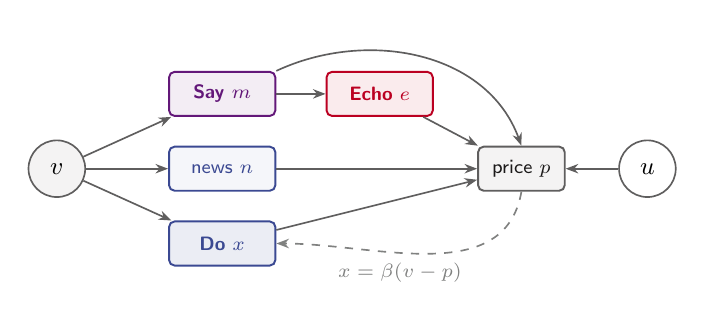
\begin{tikzpicture}[
  lat/.style={circle, draw=ink!70, line width=0.6pt, minimum size=0.72cm, font=\small, fill=ink!5},
  obs/.style={rectangle, rounded corners=2pt, line width=0.7pt, minimum width=1.35cm, minimum height=0.56cm, align=center, font=\sffamily\scriptsize},
  arr/.style={-{Stealth[length=1.6mm]}, line width=0.6pt, ink!70}]
\node[lat] (v) at (0,0) {$v$};
\node[obs, draw=say, fill=say!8, text=say] (m) at (2.1,0.95) {\textbf{Say} $m$};
\node[obs, draw=do, fill=do!5, text=do] (n) at (2.1,0) {news $n$};
\node[obs, draw=do, fill=do!10, text=do] (x) at (2.1,-0.95) {\textbf{Do} $x$};
\node[obs, draw=echo, fill=echo!8, text=echo] (e) at (4.1,0.95) {\textbf{Echo} $e$};
\node[obs, draw=ink!70, fill=ink!5, text=ink, minimum width=1.1cm] (p) at (5.9,0) {price $p$};
\node[lat, fill=white] (u) at (7.5,0) {$u$};
\draw[arr] (v) -- (m); \draw[arr] (v) -- (n); \draw[arr] (v) -- (x);
\draw[arr] (m) -- (e);
\draw[arr] (e) -- (p); \draw[arr] (n) -- (p); \draw[arr] (x) -- (p); \draw[arr] (u) -- (p);
\draw[arr] (m.north east) to[out=25,in=110] (p.north);
\draw[arr, dashed, sGray] (p.south) to[out=-100,in=0] node[below, lbl, text=sGray, pos=0.6] {$x=\beta(v-p)$} (x.east);
\end{tikzpicture}
\caption{\textbf{Information structure.} Echo is a downstream garbling of institutional speech, news is an independent signal of value, and informed demand responds to the price (dashed).}
\label{fig:dag}
\end{figure}

\subsection{Follow or fade}

\begin{theorem}[Follow-or-fade]\label{thm:followfade}
Under \cref{ass:signals,ass:price}, $\E[r\mid\y]=\kappa(\w^\star-\bphi)^\top\y$ and $\Var(r\mid\y)=\kappa^2(\sigma^2_{v|y}+\lambda^2\sigma_u^2)\eqqcolon\varsigma^2$. The loading on channel $k$ is negative (\emph{fade}) iff $\varphi_k>w^\star_k$.
\end{theorem}

\begin{corollary}[Fade the echo]\label{cor:echo}
If $e=\bm a^\top\y_{-e}+\xi$ with $\xi$ independent noise of positive variance, then $w^\star_e=0$, and the loading on $e$ is exactly $-\kappa\varphi_e$.
\end{corollary}

\begin{corollary}[Follow the news]\label{cor:news}
If $n=v+\nu_n$ with independent noise $\nu_n$, then $w^\star_n\in(0,1)$, and returns drift with $n$ whenever $\varphi_n<w^\star_n$.
\end{corollary}

\subsection{Deeds over words}

\begin{theorem}[Say--Do gap optimality]\label{thm:saydo}
Suppose a positioning proxy $\hat x=x+\xi_x$ with $\Var\xi_x=\sigma_x^2$ is also observed. Let $c_x=\beta\varsigma^2/(\beta^2\varsigma^2+\sigma_x^2)$ and $\theta=\sigma_x^2/(\beta^2\varsigma^2+\sigma_x^2)$. Then
\[
  \E[r\mid\y,\hat x]=\theta\kappa(\w^\star-\bphi)^\top\y+c_x\hat x,\quad \Var(r\mid\y,\hat x)=\theta\varsigma^2 .
\]
If the \SAY\ channel $m=y_1$ is overweighted ($\varphi_1>w^\star_1$), the forecast depends on $(m,\hat x)$ only through $-c_x(\gamma m-\hat x)$, with $\gamma=\theta\kappa(\varphi_1-w^\star_1)/c_x>0$.
\end{theorem}

\subsection{Absorption: informed or noise?}\label{sec:absorption}

The \emph{absorption} of a narrative is the price move net of the narrative-implied move, $a=p-\bphi^\top\y$.

\begin{theorem}[Absorption sign]\label{thm:absorption}
$\E[r\mid\y,a]=\E[r\mid\y]+c_A(a-\E[a\mid\y])$ with
\[
  c_A=\frac{\beta\sigma^2_{v|y}-\lambda\sigma_u^2}{\lambda(\beta^2\sigma^2_{v|y}+\sigma_u^2)} .
\]
Absorption predicts continuation iff $\beta\sigma^2_{v|y}>\lambda\sigma_u^2$, and reversal otherwise. The limits are $c_A=1/(\lambda\beta)$ as $\sigma_u\to0$ and $c_A=-1$ as $\beta\to0$.
\end{theorem}

\begin{lemma}[Robustness]\label{lem:robust}
For any $\hat\bphi$, $\hat a=p-\hat\bphi^\top\y$ generates the same $\sigma$-field as $a$ given $\y$, so $\E[r\mid\y,\hat a]=\E[r\mid\y,a]$.
\end{lemma}

At Kyle's equilibrium intensities \citep{kyle1985}, $c_A=\tfrac12$. \Cref{thm:absorption} is in the spirit of \citet{llorente2002}, but it conditions on the \emph{narrative} (\cref{fig:absorb}). In practice, the narrative-implied move comes from the embedding-based interpretation model of \cref{sec:embeddings}, and \cref{lem:robust} protects the signal against misestimating it.

\begin{figure}[t]
\centering
\begin{minipage}[t]{0.43\columnwidth}
\panel{a}
\centering
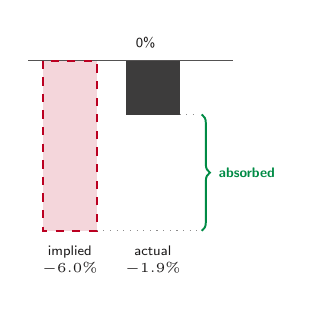
\begin{tikzpicture}[xscale=0.31, yscale=0.36]
\draw[ink!75, line width=0.5pt] (0,0) -- (8.4,0);
\node[lbl, anchor=south west, font=\sffamily\tiny] at (4.0,0.1) {0\%};
\fill[echo!16] (0.6,0) rectangle (2.8,-6);
\draw[echo, line width=0.7pt, dashed] (0.6,0) rectangle (2.8,-6);
\fill[ink!85] (4.0,0) rectangle (6.2,-1.9);
\node[lbl, align=center, anchor=north, font=\sffamily\tiny] at (1.7,-6.2) {implied\\ $-6.0\%$};
\node[lbl, align=center, anchor=north, font=\sffamily\tiny] at (5.1,-6.2) {actual\\ $-1.9\%$};
\draw[ink!50, dotted] (2.8,-6) -- (7.0,-6);
\draw[ink!50, dotted] (6.2,-1.9) -- (7.0,-1.9);
\draw[decorate, decoration={brace, amplitude=3pt, mirror}, line width=0.7pt, good] (7.1,-6) -- (7.1,-1.9);
\node[lbl, text=good, anchor=west, align=left, font=\sffamily\tiny\bfseries] at (7.4,-3.95) {absorbed};
\end{tikzpicture}
\end{minipage}\hfill
\begin{minipage}[t]{0.55\columnwidth}
\panel{b}
\centering
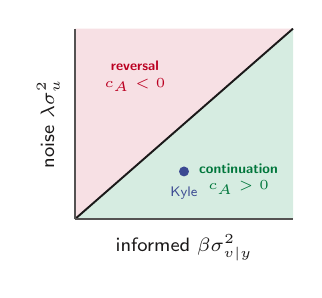
\begin{tikzpicture}
\begin{axis}[sci, width=4.35cm, height=4.0cm, xmin=0, xmax=2, ymin=0, ymax=2,
  xlabel={informed $\beta\sigma^2_{v|y}$}, ylabel={noise $\lambda\sigma_u^2$},
  xtick=\empty, ytick=\empty, clip=false, axis on top]
\addplot[name path=diag, ink, line width=0.7pt, domain=0:2] {x};
\addplot[name path=bottom, draw=none, domain=0:2] {0};
\addplot[name path=top, draw=none, domain=0:2] {2};
\addplot[good!16] fill between[of=diag and bottom];
\addplot[echo!12] fill between[of=top and diag];
\node[lbl, text=good!85!black, align=center, font=\sffamily\tiny\bfseries] at (axis cs:1.5,0.42) {continuation\\ $c_A>0$};
\node[lbl, text=echo, align=center, font=\sffamily\tiny\bfseries] at (axis cs:0.55,1.5) {reversal\\ $c_A<0$};
\fill[do] (axis cs:1,0.5) circle (1.8pt);
\node[lbl, text=do, anchor=north, font=\sffamily\tiny] at (axis cs:1,0.44) {Kyle};
\end{axis}
\end{tikzpicture}
\end{minipage}
\caption{\textbf{Absorption.} \textbf{a},~The narrative implied a 6\% fall; the price fell 1.9\%. \textbf{b},~Phase diagram of \cref{thm:absorption}: absorption signals a hidden buyer only where informed intensity dominates noise.}
\label{fig:absorb}
\end{figure}

% =====================================================================
\section{Strategic Speech and False Alarms}\label{sec:strategic}

We now let the institution \emph{choose} what to say.

\begin{assumption}[Strategic institution]\label{ass:strategic}
An institution knows $v$, which may have any distribution with mean $0$ and variance $\sigma_v^2<\infty$. It publishes $m$ and trades $x$. The public sees $\tilde m=m+\varepsilon$, where $\varepsilon$ has mean zero and variance $\sigma_\varepsilon^2$ and is independent of $v$. The price is $p=\varphi\tilde m+\lambda x$, where $\varphi\ge0$ is the crowd's \emph{credulity}. Misreporting costs $\tfrac k2(m-v)^2$. The institution maximises $J=x(v-\varphi m-\lambda x)-\tfrac k2(m-v)^2$. Let $a\coloneqq2\lambda k$.
\end{assumption}

\begin{assumption}[Echo amplification]\label{ass:amplify}
Each article moves the price by $\varphi_0$ per unit of message, and a Hawkes cascade with branching ratio $n\in[0,1)$ repeats it. Hence $\varphi=\varphi_0/(1-n)$ (\cref{prop:branching}).
\end{assumption}

\begin{theorem}[Optimal speech and trade]\label{thm:speech}
$J$ has a unique maximiser iff $a>\varphi^2$, namely $m^\ast=\psi v$ and $x^\ast=\chi v$ with
\[
  \psi=\frac{a-\varphi}{a-\varphi^2},\qquad \chi=\frac{k(1-\varphi)}{a-\varphi^2}.
\]
If $a<\varphi^2$, $J$ is unbounded: only position limits contain manipulation.
\end{theorem}

\begin{corollary}[Taxonomy]\label{cor:taxonomy}
Let $a>\varphi^2$ and $v>0$. The institution tells the \textbf{truth} if $\varphi=1$. It \textbf{shades} ($0<\psi<1$, buys) if $\varphi<1<a/\varphi$. It raises a \textbf{false alarm} ($\psi<0<\chi$: talks down, buys) if $\varphi^2<a<\varphi<1$. It \textbf{exaggerates and sells} ($\psi>1$, $\chi<0$) if $\varphi>1$.
\end{corollary}

\begin{theorem}[Say--Do covariance identity]\label{thm:identity}
Under \cref{ass:strategic}, let the message rule $m(v)$ be \emph{arbitrary} and the trade optimal given it. Then, pathwise, $r=\lambda x-\varphi\varepsilon$. Hence, for any law of $v$,
\[
  \Cov(r,\tilde m)=\lambda\Cov(x,\tilde m)-\varphi\sigma_\varepsilon^2,\qquad \E[r\mid x]=\lambda x.
\]
In equilibrium, $\Cov(x,\tilde m)=\psi\chi\sigma_v^2$, which is negative exactly in the false-alarm and exaggeration regimes.
\end{theorem}

\begin{takeaway}{Why it matters.}
Both sides of the identity are estimable, and no distributional assumption is needed. The rolling sign of $\widehat{\Cov}(\text{Say},\text{Do})$ tells the econometrician whether to follow or fade institutional words, while deeds are always followed, with slope $\lambda$.
\end{takeaway}

\begin{proposition}[Manipulation dichotomy]\label{prop:virality}
Under \cref{ass:strategic,ass:amplify} with $\varphi_0\in(0,1)$, call a regime manipulative if $\Cov(\text{Say},\text{Do})<0$. \textup{(i)}~If $a<1$ (a deep market), the only manipulative regime is the false alarm, which occurs iff $\max\{0,1-\varphi_0/a\}<n<1-\varphi_0/\sqrt a$. \textup{(ii)}~If $a>1$ (a shallow market), it is exaggeration, which occurs iff $1-\varphi_0<n<1-\varphi_0/\sqrt a$. \textup{(iii)}~For $n>1-\varphi_0/\sqrt a$ no interior optimum exists.
\end{proposition}

\paragraph{Adaptive trust} Suppose the crowd resets its credulity each round to the least-squares slope of value on message under the previous strategy, a cobweb rule \citep{ezekiel1938,evans2001}. This gives $\varphi_{t+1}=1/\psi(\varphi_t)=F_a(\varphi_t)$ with $F_a(\varphi)=(a-\varphi^2)/(a-\varphi)$.

\begin{theorem}[Credibility cycles]\label{thm:cycles}
\textup{(i)}~For $a>1$, truth ($\varphi=1$) is the unique admissible fixed point. \textup{(ii)}~$F_a'(1)=-1/(a-1)$, so truth is stable iff $\lambda k>1$. \textup{(iii)}~For $1<a<2$ there is exactly one $2$-cycle,
\[
  \varphi_\pm=\tfrac12\big(a\pm\sqrt{a(2-a)}\big),\qquad \varphi_-<1<\varphi_+,
\]
with multiplier $(5a-9)/(a-1)$. It is stable iff $\tfrac56<\lambda k<1$, and it alternates between shading and exaggeration. \textup{(iv)}~The cycle is born by a flip at $a=2$ and loses stability by a second flip at $a=\tfrac53$.
\end{theorem}

\begin{figure*}[t]
\centering
\begin{minipage}[t]{0.325\textwidth}
\panel{a}
\centering
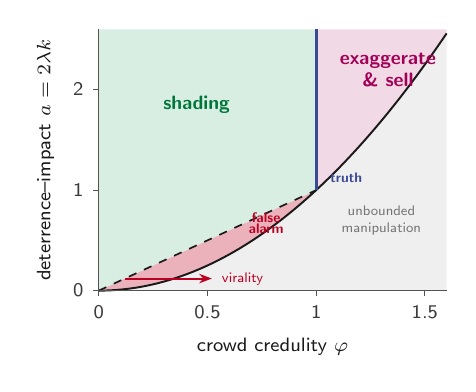
\begin{tikzpicture}
\begin{axis}[sci, width=6.0cm, height=4.9cm, xmin=0, xmax=1.6, ymin=0, ymax=2.6,
  xlabel={crowd credulity $\varphi$}, ylabel={deterrence--impact $a=2\lambda k$},
  xtick={0,0.5,1,1.5}, ytick={0,1,2}, axis on top, clip=false]
\addplot[name path=sq, ink, line width=0.7pt, domain=0:1.6, samples=60] {x^2};
\addplot[name path=lin, ink, line width=0.6pt, dashed, domain=0:1, samples=2] {x};
\addplot[name path=top, draw=none, domain=0:1.6, samples=2] {2.6};
\addplot[name path=bot, draw=none, domain=0:1.6, samples=2] {0};
\addplot[ink!7] fill between[of=sq and bot];
\addplot[echo!30] fill between[of=lin and sq, soft clip={domain=0:1}];
\addplot[good!15] fill between[of=top and lin, soft clip={domain=0:1}];
\addplot[sMagenta!15] fill between[of=top and sq, soft clip={domain=1:1.6}];
\draw[do, line width=1.2pt] (axis cs:1,1) -- (axis cs:1,2.6);
\node[lbl, text=good!85!black, font=\sffamily\scriptsize\bfseries] at (axis cs:0.45,1.85) {shading};
\node[lbl, text=echo, font=\sffamily\tiny\bfseries, align=center] at (axis cs:0.77,0.67) {false\\[-2pt]alarm};
\node[lbl, text=sMagenta, font=\sffamily\scriptsize\bfseries, align=center] at (axis cs:1.33,2.2) {exaggerate\\ \& sell};
\node[lbl, text=ink!60, font=\sffamily\tiny, align=center] at (axis cs:1.3,0.7) {unbounded\\ manipulation};
\node[lbl, text=do, font=\sffamily\tiny\bfseries, anchor=west] at (axis cs:1.02,1.12) {truth};
\draw[-{Stealth[length=1.6mm]}, echo, line width=0.7pt] (axis cs:0.12,0.12) -- (axis cs:0.52,0.12) node[right, lbl, text=echo, font=\sffamily\tiny] {virality};
\end{axis}
\end{tikzpicture}
\end{minipage}\hfill
\begin{minipage}[t]{0.325\textwidth}
\panel{b}
\centering
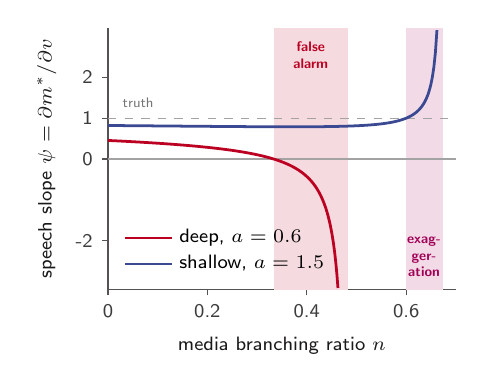
\begin{tikzpicture}
\begin{axis}[sci, width=6.0cm, height=4.9cm, xmin=0, xmax=0.7, ymin=-3.2, ymax=3.2,
  xlabel={media branching ratio $n$}, ylabel={speech slope $\psi=\partial m^\ast/\partial v$},
  xtick={0,0.2,0.4,0.6}, ytick={-2,0,1,2}, unbounded coords=jump,
  legend style={at={(0.02,0.02)}, anchor=south west}]
\fill[echo!14] (axis cs:0.3333,-3.2) rectangle (axis cs:0.4836,3.2);
\fill[sMagenta!14] (axis cs:0.6,-3.2) rectangle (axis cs:0.6734,3.2);
\addplot[ink!40, line width=0.4pt, forget plot] coordinates {(0,0) (0.7,0)};
\addplot[ink!40, line width=0.4pt, dashed, forget plot] coordinates {(0,1) (0.7,1)};
\addplot[echo, domain=0:0.478, samples=220, restrict y to domain=-3.3:3.3] {(0.6-0.4/(1-x))/(0.6-(0.4/(1-x))^2)};
\addlegendentry{deep, $a=0.6$}
\addplot[do, domain=0:0.668, samples=220, restrict y to domain=-3.3:3.3] {(1.5-0.4/(1-x))/(1.5-(0.4/(1-x))^2)};
\addlegendentry{shallow, $a=1.5$}
\node[lbl, text=echo, font=\sffamily\tiny\bfseries, align=center] at (axis cs:0.408,2.55) {false\\ alarm};
\node[lbl, text=sMagenta, font=\sffamily\tiny\bfseries, align=center] at (axis cs:0.636,-2.4) {exag-\\ger-\\ation};
\node[lbl, text=ink!60, font=\sffamily\tiny, anchor=south west] at (axis cs:0.01,1.02) {truth};
\end{axis}
\end{tikzpicture}
\end{minipage}\hfill
\begin{minipage}[t]{0.325\textwidth}
\panel{c}
\centering
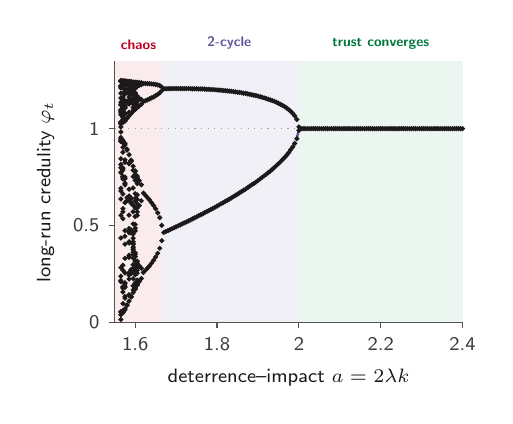
\begin{tikzpicture}
\begin{axis}[sci, width=6.0cm, height=4.9cm, xmin=1.55, xmax=2.4, ymin=0, ymax=1.35,
  xlabel={deterrence--impact $a=2\lambda k$}, ylabel={long-run credulity $\varphi_t$},
  xtick={1.6,1.8,2,2.2,2.4}, ytick={0,0.5,1}, clip=false]
\fill[echo!8] (axis cs:1.55,0) rectangle (axis cs:1.6667,1.35);
\fill[sViolet!9] (axis cs:1.6667,0) rectangle (axis cs:2,1.35);
\fill[good!8] (axis cs:2,0) rectangle (axis cs:2.4,1.35);
\addplot[only marks, mark=*, mark size=0.28pt, ink] coordinates {(1.565,0.014) (1.565,0.039) (1.565,0.053) (1.565,0.054) (1.565,0.209) (1.565,0.216) (1.565,0.238) (1.565,0.282) (1.565,0.435) (1.565,0.552) (1.565,0.637) (1.565,0.678) (1.565,0.692) (1.565,0.772) (1.565,0.775) (1.565,0.798) (1.565,0.815) (1.565,0.844) (1.565,0.934) (1.565,0.935) (1.565,0.941) (1.565,0.946) (1.565,0.954) (1.565,0.983) (1.565,1.009) (1.565,1.024) (1.565,1.028) (1.565,1.03) (1.565,1.033) (1.565,1.034) (1.565,1.072) (1.565,1.082) (1.565,1.089) (1.565,1.096) (1.565,1.097) (1.565,1.122) (1.565,1.126) (1.565,1.137) (1.565,1.158) (1.565,1.183) (1.565,1.21) (1.565,1.217) (1.565,1.221) (1.565,1.222) (1.565,1.244) (1.565,1.246) (1.565,1.249) (1.57,0.049) (1.57,0.05) (1.57,0.06) (1.57,0.096) (1.57,0.156) (1.57,0.176) (1.57,0.178) (1.57,0.184) (1.57,0.268) (1.57,0.294) (1.57,0.535) (1.57,0.571) (1.57,0.587) (1.57,0.662) (1.57,0.74) (1.57,0.75) (1.57,0.751) (1.57,0.753) (1.57,0.786) (1.57,0.796) (1.57,0.878) (1.57,0.903) (1.57,0.927) (1.57,0.94) (1.57,1.032) (1.57,1.037) (1.57,1.048) (1.57,1.059) (1.57,1.09) (1.57,1.093) (1.57,1.104) (1.57,1.105) (1.57,1.108) (1.57,1.131) (1.57,1.151) (1.57,1.154) (1.57,1.163) (1.57,1.21) (1.57,1.214) (1.57,1.228) (1.57,1.229) (1.57,1.232) (1.57,1.24) (1.57,1.245) (1.57,1.246) (1.57,1.247) (1.575,0.063) (1.575,0.069) (1.575,0.124) (1.575,0.133) (1.575,0.18) (1.575,0.185) (1.575,0.199) (1.575,0.204) (1.575,0.255) (1.575,0.33) (1.575,0.403) (1.575,0.444) (1.575,0.473) (1.575,0.618) (1.575,0.709) (1.575,0.715) (1.575,0.719) (1.575,0.741) (1.575,0.744) (1.575,0.75) (1.575,0.826) (1.575,0.839) (1.575,0.916) (1.575,0.924) (1.575,1.039) (1.575,1.043) (1.575,1.075) (1.575,1.08) (1.575,1.106) (1.575,1.108) (1.575,1.109) (1.575,1.116) (1.575,1.117) (1.575,1.119) (1.575,1.144) (1.575,1.178) (1.575,1.184) (1.575,1.192) (1.575,1.205) (1.575,1.218) (1.575,1.226) (1.575,1.227) (1.575,1.229) (1.575,1.23) (1.575,1.237) (1.575,1.238) (1.575,1.246) (1.575,1.247) (1.58,0.087) (1.58,0.09) (1.58,0.628) (1.58,0.644) (1.58,0.889) (1.58,0.894) (1.58,1.053) (1.58,1.055) (1.58,1.138) (1.58,1.142) (1.58,1.245) (1.585,0.109) (1.585,0.139) (1.585,0.14) (1.585,0.141) (1.585,0.223) (1.585,0.243) (1.585,0.256) (1.585,0.335) (1.585,0.342) (1.585,0.346) (1.585,0.409) (1.585,0.412) (1.585,0.416) (1.585,0.462) (1.585,0.471) (1.585,0.484) (1.585,0.553) (1.585,0.629) (1.585,0.652) (1.585,0.687) (1.585,0.819) (1.585,0.82) (1.585,0.821) (1.585,0.865) (1.585,1.066) (1.585,1.083) (1.585,1.084) (1.585,1.127) (1.585,1.137) (1.585,1.143) (1.585,1.162) (1.585,1.178) (1.585,1.181) (1.585,1.183) (1.585,1.192) (1.585,1.193) (1.585,1.194) (1.585,1.206) (1.585,1.208) (1.585,1.221) (1.585,1.224) (1.585,1.227) (1.585,1.239) (1.585,1.24) (1.585,1.244) (1.59,0.13) (1.59,0.131) (1.59,0.132) (1.59,0.133) (1.59,0.252) (1.59,0.254) (1.59,0.264) (1.59,0.268) (1.59,0.272) (1.59,0.462) (1.59,0.465) (1.59,0.467) (1.59,0.474) (1.59,0.476) (1.59,0.614) (1.59,0.621) (1.59,0.638) (1.59,0.642) (1.59,0.832) (1.59,0.833) (1.59,0.834) (1.59,0.836) (1.59,0.837) (1.59,1.078) (1.59,1.079) (1.59,1.141) (1.59,1.142) (1.59,1.147) (1.59,1.148) (1.59,1.181) (1.59,1.182) (1.59,1.183) (1.59,1.184) (1.59,1.22) (1.59,1.221) (1.59,1.222) (1.59,1.223) (1.59,1.224) (1.59,1.242) (1.59,1.243) (1.595,0.153) (1.595,0.167) (1.595,0.188) (1.595,0.225) (1.595,0.278) (1.595,0.297) (1.595,0.332) (1.595,0.349) (1.595,0.361) (1.595,0.374) (1.595,0.384) (1.595,0.388) (1.595,0.402) (1.595,0.408) (1.595,0.416) (1.595,0.434) (1.595,0.456) (1.595,0.508) (1.595,0.571) (1.595,0.604) (1.595,0.693) (1.595,0.752) (1.595,0.785) (1.595,0.806) (1.595,1.09) (1.595,1.097) (1.595,1.109) (1.595,1.127) (1.595,1.152) (1.595,1.161) (1.595,1.176) (1.595,1.187) (1.595,1.192) (1.595,1.195) (1.595,1.197) (1.595,1.198) (1.595,1.201) (1.595,1.202) (1.595,1.204) (1.595,1.206) (1.595,1.208) (1.595,1.212) (1.595,1.218) (1.595,1.221) (1.595,1.23) (1.595,1.236) (1.595,1.239) (1.595,1.241) (1.6,0.171) (1.6,0.173) (1.6,0.184) (1.6,0.203) (1.6,0.246) (1.6,0.26) (1.6,0.269) (1.6,0.289) (1.6,0.315) (1.6,0.339) (1.6,0.35) (1.6,0.358) (1.6,0.472) (1.6,0.486) (1.6,0.505) (1.6,0.546) (1.6,0.591) (1.6,0.625) (1.6,0.64) (1.6,0.664) (1.6,0.733) (1.6,0.763) (1.6,0.779) (1.6,0.782) (1.6,1.099) (1.6,1.1) (1.6,1.106) (1.6,1.116) (1.6,1.137) (1.6,1.144) (1.6,1.148) (1.6,1.157) (1.6,1.168) (1.6,1.178) (1.6,1.182) (1.6,1.185) (1.6,1.208) (1.6,1.21) (1.6,1.212) (1.6,1.216) (1.6,1.221) (1.6,1.224) (1.6,1.226) (1.6,1.228) (1.6,1.235) (1.6,1.238) (1.6,1.24) (1.605,0.191) (1.605,0.195) (1.605,0.2) (1.605,0.205) (1.605,0.21) (1.605,0.217) (1.605,0.253) (1.605,0.267) (1.605,0.281) (1.605,0.293) (1.605,0.306) (1.605,0.316) (1.605,0.552) (1.605,0.57) (1.605,0.59) (1.605,0.612) (1.605,0.635) (1.605,0.658) (1.605,0.716) (1.605,0.726) (1.605,0.735) (1.605,0.742) (1.605,0.749) (1.605,0.755) (1.605,1.109) (1.605,1.111) (1.605,1.114) (1.605,1.116) (1.605,1.119) (1.605,1.122) (1.605,1.14) (1.605,1.146) (1.605,1.152) (1.605,1.158) (1.605,1.163) (1.605,1.168) (1.605,1.218) (1.605,1.22) (1.605,1.222) (1.605,1.224) (1.605,1.226) (1.605,1.229) (1.605,1.235) (1.605,1.236) (1.605,1.237) (1.605,1.238) (1.605,1.239) (1.61,0.21) (1.61,0.291) (1.61,0.602) (1.61,0.731) (1.61,1.118) (1.61,1.156) (1.61,1.224) (1.61,1.238) (1.615,0.226) (1.615,0.279) (1.615,0.627) (1.615,0.71) (1.615,1.126) (1.615,1.151) (1.615,1.228) (1.615,1.237) (1.62,0.257) (1.62,0.667) (1.62,1.14) (1.62,1.233) (1.625,0.268) (1.625,0.656) (1.625,1.144) (1.625,1.233) (1.63,0.279) (1.63,0.644) (1.63,1.149) (1.63,1.233) (1.635,0.291) (1.635,0.632) (1.635,1.154) (1.635,1.232) (1.64,0.305) (1.64,0.618) (1.64,1.159) (1.64,1.231) (1.645,0.32) (1.645,0.603) (1.645,1.164) (1.645,1.23) (1.65,0.337) (1.65,0.586) (1.65,1.17) (1.65,1.228) (1.655,0.356) (1.655,0.565) (1.655,1.177) (1.655,1.226) (1.66,0.382) (1.66,0.54) (1.66,1.185) (1.66,1.222) (1.665,0.421) (1.665,0.5) (1.665,1.196) (1.665,1.215) (1.67,0.464) (1.67,1.206) (1.675,0.469) (1.675,1.206) (1.68,0.473) (1.68,1.207) (1.685,0.478) (1.685,1.207) (1.69,0.483) (1.69,1.207) (1.695,0.488) (1.695,1.207) (1.7,0.493) (1.7,1.207) (1.705,0.498) (1.705,1.207) (1.71,0.503) (1.71,1.207) (1.715,0.508) (1.715,1.207) (1.72,0.513) (1.72,1.207) (1.725,0.518) (1.725,1.207) (1.73,0.523) (1.73,1.207) (1.735,0.528) (1.735,1.207) (1.74,0.534) (1.74,1.206) (1.745,0.539) (1.745,1.206) (1.75,0.544) (1.75,1.206) (1.755,0.55) (1.755,1.205) (1.76,0.555) (1.76,1.205) (1.765,0.56) (1.765,1.205) (1.77,0.566) (1.77,1.204) (1.775,0.572) (1.775,1.203) (1.78,0.577) (1.78,1.203) (1.785,0.583) (1.785,1.202) (1.79,0.588) (1.79,1.202) (1.795,0.594) (1.795,1.201) (1.8,0.6) (1.8,1.2) (1.805,0.606) (1.805,1.199) (1.81,0.612) (1.81,1.198) (1.815,0.618) (1.815,1.197) (1.82,0.624) (1.82,1.196) (1.825,0.63) (1.825,1.195) (1.83,0.636) (1.83,1.194) (1.835,0.642) (1.835,1.193) (1.84,0.649) (1.84,1.191) (1.845,0.655) (1.845,1.19) (1.85,0.662) (1.85,1.188) (1.855,0.668) (1.855,1.187) (1.86,0.675) (1.86,1.185) (1.865,0.682) (1.865,1.183) (1.87,0.688) (1.87,1.182) (1.875,0.695) (1.875,1.18) (1.88,0.703) (1.88,1.177) (1.885,0.71) (1.885,1.175) (1.89,0.717) (1.89,1.173) (1.895,0.724) (1.895,1.171) (1.9,0.732) (1.9,1.168) (1.905,0.74) (1.905,1.165) (1.91,0.748) (1.91,1.162) (1.915,0.756) (1.915,1.159) (1.92,0.764) (1.92,1.156) (1.925,0.773) (1.925,1.152) (1.93,0.781) (1.93,1.149) (1.935,0.79) (1.935,1.145) (1.94,0.799) (1.94,1.141) (1.945,0.809) (1.945,1.136) (1.95,0.819) (1.95,1.131) (1.955,0.829) (1.955,1.126) (1.96,0.84) (1.96,1.12) (1.965,0.851) (1.965,1.114) (1.97,0.863) (1.97,1.107) (1.975,0.876) (1.975,1.099) (1.98,0.891) (1.98,1.089) (1.985,0.906) (1.985,1.079) (1.99,0.924) (1.99,1.066) (1.995,0.948) (1.995,1.047) (2.0,0.991) (2.0,1.009) (2.005,1.0) (2.01,1.0) (2.015,1.0) (2.02,1.0) (2.025,1.0) (2.03,1.0) (2.035,1.0) (2.04,1.0) (2.045,1.0) (2.05,1.0) (2.055,1.0) (2.06,1.0) (2.065,1.0) (2.07,1.0) (2.075,1.0) (2.08,1.0) (2.085,1.0) (2.09,1.0) (2.095,1.0) (2.1,1.0) (2.105,1.0) (2.11,1.0) (2.115,1.0) (2.12,1.0) (2.125,1.0) (2.13,1.0) (2.135,1.0) (2.14,1.0) (2.145,1.0) (2.15,1.0) (2.155,1.0) (2.16,1.0) (2.165,1.0) (2.17,1.0) (2.175,1.0) (2.18,1.0) (2.185,1.0) (2.19,1.0) (2.195,1.0) (2.2,1.0) (2.205,1.0) (2.21,1.0) (2.215,1.0) (2.22,1.0) (2.225,1.0) (2.23,1.0) (2.235,1.0) (2.24,1.0) (2.245,1.0) (2.25,1.0) (2.255,1.0) (2.26,1.0) (2.265,1.0) (2.27,1.0) (2.275,1.0) (2.28,1.0) (2.285,1.0) (2.29,1.0) (2.295,1.0) (2.3,1.0) (2.305,1.0) (2.31,1.0) (2.315,1.0) (2.32,1.0) (2.325,1.0) (2.33,1.0) (2.335,1.0) (2.34,1.0) (2.345,1.0) (2.35,1.0) (2.355,1.0) (2.36,1.0) (2.365,1.0) (2.37,1.0) (2.375,1.0) (2.38,1.0) (2.385,1.0) (2.39,1.0) (2.395,1.0) (2.4,1.0)};
\addplot[sViolet, line width=0.9pt, dashed, domain=1.6667:2, samples=60] {(x+sqrt(x*(2-x)))/2};
\addplot[sViolet, line width=0.9pt, dashed, domain=1.6667:2, samples=60] {(x-sqrt(x*(2-x)))/2};
\addplot[ink!40, line width=0.4pt, dotted] coordinates {(1.55,1) (2.4,1)};
\node[lbl, text=good!85!black, font=\sffamily\tiny\bfseries, anchor=south] at (axis cs:2.2,1.36) {trust converges};
\node[lbl, text=sViolet, font=\sffamily\tiny\bfseries, anchor=south] at (axis cs:1.83,1.36) {2-cycle};
\node[lbl, text=echo, font=\sffamily\tiny\bfseries, anchor=south] at (axis cs:1.608,1.36) {chaos};
\end{axis}
\end{tikzpicture}
\end{minipage}
\caption{\textbf{The economics of false alarms.} \textbf{a},~Regime map (\cref{thm:speech,cor:taxonomy}). False alarms occupy the wedge $\varphi^2<a<\varphi$; echo amplification moves the market to the right. \textbf{b},~Speech slope against the media echo share (\cref{prop:virality}, $\varphi_0=0.4$). Deep markets pass through a false-alarm window ($\psi<0$); shallow markets pass through an exaggeration window ($\psi>1$). \textbf{c},~Bifurcation diagram of adaptive trust (\cref{thm:cycles}). Dots show the long-run attractor, and dashed curves the closed-form cycle $\varphi_\pm$. Trust converges for $a>2$, cycles for $\tfrac53<a<2$, and becomes chaotic below (numerical Lyapunov exponent $\approx0.10$ at $a=1.6$).}
\label{fig:strategic}
\end{figure*}

\paragraph{Relation to prior work} \citet{benabou1992} derive credibility dynamics from Bayesian learning about a random honest type, and \citet{kartik2007} study costly talk with credulous receivers. Our contribution is a trading-coupled linear--quadratic model in which the false-alarm region, the Say--Do covariance identity and the bifurcation thresholds are all explicit and estimable.

% =====================================================================
\section{Measuring the Voices}\label{sec:measure}

\subsection{Echo: exact semantic declustering}\label{sec:echo}

Articles arrive at times $\tau_1<\dots<\tau_N$ with embeddings $\z_j$ and a Hawkes intensity $\lambda(t)=\mu+\sum_{\tau_l<t}g(t-\tau_l)$ with $n=\int g<1$. In the cluster representation \citep{hawkesoakes1974}, each article is either news (an immigrant) or an echo of an earlier article.

\begin{proposition}[Echo share]\label{prop:branching}
In stationarity, the long-run share of articles that are echoes equals the branching ratio $n$, and the mean cascade size is $(1-n)^{-1}$.
\end{proposition}

\begin{assumption}[Marked cascade]\label{ass:marked}
News embeddings are i.i.d.\ with density $f_0$. An echo of article $l$ has density $f(\cdot\mid\z_l)$, for example von Mises--Fisher, $f\propto e^{\varkappa\langle\z,\z_l\rangle}$.
\end{assumption}

\begin{theorem}[Semantic declustering]\label{thm:semantic}
Given all times and embeddings on $[0,T]$, the parent labels $\pi(j)$ are independent, with
\begin{gather*}
  \Prob(\pi(j)=0\mid\cdot)=\frac{\mu f_0(\z_j)}{\Lambda_j},\\
  \Prob(\pi(j)=l\mid\cdot)=\frac{g(\tau_j-\tau_l)f(\z_j\mid\z_l)}{\Lambda_j},
\end{gather*}
where $\Lambda_j=\mu f_0(\z_j)+\sum_{l<j}g(\tau_j-\tau_l)f(\z_j\mid\z_l)$. The MMSE split of sentiment $s_j=\langle\w_s,\z_j\rangle$ is $s^{\mathrm{new}}=\sum_jp^{\mathrm{sem}}_js_j$ and $s^{\mathrm{echo}}=\sum_j(1-p^{\mathrm{sem}}_j)s_j$, with $p^{\mathrm{sem}}_j=\mu f_0(\z_j)/\Lambda_j$. Semantics never increases the expected posterior entropy of parentage relative to timing alone.
\end{theorem}

Setting $f\equiv f_0$ recovers timing-only stochastic declustering \citep{zhuang2002}, where $p_j=\mu/\lambda(\tau_j)$. Combined with \cref{cor:echo}, $s^{\mathrm{echo}}$ estimates exactly the garbled component that the crowd should not have priced (\cref{fig:echo}).

\begin{figure*}[t]
\centering
\begin{minipage}[t]{0.53\textwidth}
\panel{a}
\centering
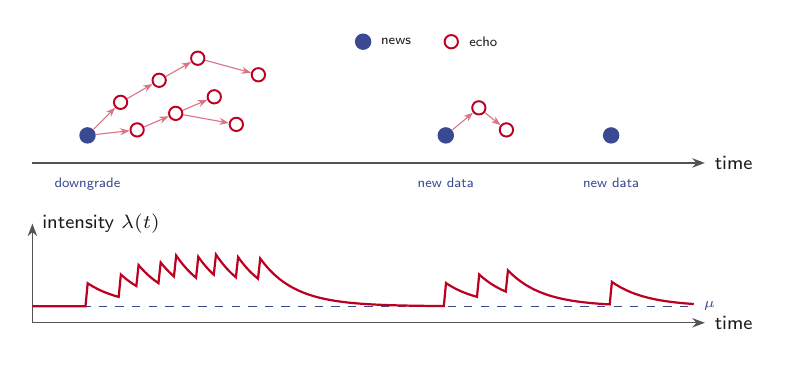
\begin{tikzpicture}[scale=0.7,
  newn/.style={circle, fill=do, inner sep=2.1pt},
  echn/.style={circle, draw=echo, line width=0.7pt, fill=white, inner sep=1.7pt},
  trig/.style={-{Stealth[length=1.2mm]}, echo!55, line width=0.4pt}]
\draw[-{Stealth[length=1.6mm]}, ink!75, line width=0.5pt] (0,0) -- (12.2,0) node[right, lbl] {time};
\node[newn] (a) at (1,0.5) {};
\node[echn] (a1) at (1.6,1.1) {}; \node[echn] (a2) at (1.9,0.6) {}; \node[echn] (a3) at (2.3,1.5) {};
\node[echn] (a4) at (2.6,0.9) {}; \node[echn] (a5) at (3.0,1.9) {}; \node[echn] (a6) at (3.3,1.2) {};
\node[echn] (a7) at (3.7,0.7) {}; \node[echn] (a8) at (4.1,1.6) {};
\draw[trig] (a) -- (a1); \draw[trig] (a) -- (a2); \draw[trig] (a1) -- (a3); \draw[trig] (a2) -- (a4);
\draw[trig] (a3) -- (a5); \draw[trig] (a4) -- (a6); \draw[trig] (a4) -- (a7); \draw[trig] (a5) -- (a8);
\node[newn] (b) at (7.5,0.5) {}; \node[echn] (b1) at (8.1,1.0) {}; \node[echn] (b2) at (8.6,0.6) {};
\draw[trig] (b) -- (b1); \draw[trig] (b1) -- (b2);
\node[newn] (c) at (10.5,0.5) {};
\node[lbl, text=do, anchor=north, font=\sffamily\tiny] at (1,-0.1) {downgrade};
\node[lbl, text=do, anchor=north, font=\sffamily\tiny] at (7.5,-0.1) {new data};
\node[lbl, text=do, anchor=north, font=\sffamily\tiny] at (10.5,-0.1) {new data};
\node[newn] at (6.0,2.2) {}; \node[lbl, anchor=west, font=\sffamily\tiny] at (6.15,2.2) {news};
\node[echn] at (7.6,2.2) {}; \node[lbl, anchor=west, font=\sffamily\tiny] at (7.75,2.2) {echo};
\begin{scope}[yshift=-2.9cm]
\draw[-{Stealth[length=1.6mm]}, ink!75, line width=0.5pt] (0,0) -- (12.2,0) node[right, lbl] {time};
\draw[-{Stealth[length=1.6mm]}, ink!75, line width=0.5pt] (0,0) -- (0,1.8) node[right, lbl] {intensity $\lambda(t)$};
\draw[dashed, do, line width=0.5pt] (0,0.3) -- (12,0.3) node[right, lbl, text=do, font=\sffamily\tiny] {$\mu$};
\draw[echo, line width=0.8pt, samples=300, domain=0:12] plot (\x, {0.3
  + 0.42*(\x>1.0)*exp(-1.6*max(\x-1.0,0)) + 0.42*(\x>1.6)*exp(-1.6*max(\x-1.6,0))
  + 0.42*(\x>1.9)*exp(-1.6*max(\x-1.9,0)) + 0.42*(\x>2.3)*exp(-1.6*max(\x-2.3,0))
  + 0.42*(\x>2.6)*exp(-1.6*max(\x-2.6,0)) + 0.42*(\x>3.0)*exp(-1.6*max(\x-3.0,0))
  + 0.42*(\x>3.3)*exp(-1.6*max(\x-3.3,0)) + 0.42*(\x>3.7)*exp(-1.6*max(\x-3.7,0))
  + 0.42*(\x>4.1)*exp(-1.6*max(\x-4.1,0)) + 0.42*(\x>7.5)*exp(-1.6*max(\x-7.5,0))
  + 0.42*(\x>8.1)*exp(-1.6*max(\x-8.1,0)) + 0.42*(\x>8.6)*exp(-1.6*max(\x-8.6,0))
  + 0.42*(\x>10.5)*exp(-1.6*max(\x-10.5,0))});
\end{scope}
\end{tikzpicture}
\end{minipage}\hfill
\begin{minipage}[t]{0.44\textwidth}
\panel{b}
\centering
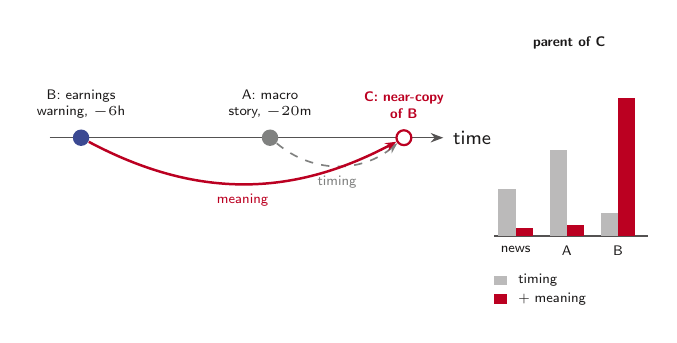
\begin{tikzpicture}[font=\sffamily]
\draw[-{Stealth[length=1.6mm]}, ink!75, line width=0.5pt] (0,0) -- (5.0,0) node[right, lbl] {time};
\node[circle, fill=do, inner sep=2.1pt] (B) at (0.4,0) {};
\node[circle, fill=sGray, inner sep=2.1pt] (A) at (2.8,0) {};
\node[circle, draw=echo, line width=0.8pt, fill=white, inner sep=1.9pt] (C) at (4.5,0) {};
\node[lbl, align=center, anchor=south, font=\sffamily\tiny] at (0.4,0.12) {B: earnings\\ warning, $-6$h};
\node[lbl, align=center, anchor=south, font=\sffamily\tiny] at (2.8,0.12) {A: macro\\ story, $-20$m};
\node[lbl, align=center, anchor=south, text=echo, font=\sffamily\tiny\bfseries] at (4.5,0.12) {C: near-copy\\ of B};
\draw[-{Stealth[length=1.4mm]}, sGray, dashed, line width=0.6pt] (A) to[out=-40,in=-140] node[below, lbl, text=sGray, font=\sffamily\tiny] {timing} (C);
\draw[-{Stealth[length=1.4mm]}, echo, line width=0.9pt] (B) to[out=-28,in=-152] node[below, lbl, text=echo, font=\sffamily\tiny] {meaning} (C);
\begin{scope}[xshift=5.65cm, yshift=-1.25cm]
\node[lbl, anchor=south, font=\sffamily\tiny\bfseries] at (0.95,2.25) {parent of C};
\draw[ink!75, line width=0.5pt] (0,0) -- (1.95,0);
\fill[ink!30] (0.05,0) rectangle (0.27,0.60); \fill[echo] (0.27,0) rectangle (0.49,0.10);
\fill[ink!30] (0.70,0) rectangle (0.92,1.10); \fill[echo] (0.92,0) rectangle (1.14,0.14);
\fill[ink!30] (1.35,0) rectangle (1.57,0.30); \fill[echo] (1.57,0) rectangle (1.79,1.76);
\node[lbl, anchor=north, font=\sffamily\tiny] at (0.27,0) {news};
\node[lbl, anchor=north, font=\sffamily\tiny] at (0.92,0) {A};
\node[lbl, anchor=north, font=\sffamily\tiny] at (1.57,0) {B};
\fill[ink!30] (0,-0.62) rectangle (0.16,-0.5); \node[lbl, anchor=west, font=\sffamily\tiny] at (0.18,-0.56) {timing};
\fill[echo] (0,-0.86) rectangle (0.16,-0.74); \node[lbl, anchor=west, font=\sffamily\tiny] at (0.18,-0.8) {+ meaning};
\end{scope}
\end{tikzpicture}
\end{minipage}
\caption{\textbf{Separating news from echo.} \textbf{a},~A news article (blue) triggers a cascade of echoes (red), and the intensity jumps and decays to the baseline $\mu$. The long-run echo share equals the branching ratio (\cref{prop:branching}). \textbf{b},~Semantic declustering (\cref{thm:semantic}; illustrative numbers). Timing alone attributes article C to the most recent story A; adding embedding similarity correctly identifies C as an echo of B.}
\label{fig:echo}
\end{figure*}

\subsection{Market-aligned embeddings}\label{sec:embeddings}

Documents are embedded on the sphere, $\z_j\in S^{D-1}$. Each has a post-event response vector $\bm\rho_j$ (multi-horizon abnormal returns, abnormal volume, change in implied volatility). Let $S_{jk}=\langle\z_j,\z_k\rangle$ and $D_{jk}=\|\bm\rho_j-\bm\rho_k\|^2$. The return-aligned soft-contrastive loss is $\mathcal{L}(Z)=-\sum_j\sum_{k\neq j}q_{jk}\log p_{jk}(Z)$, where
\[
  q_{jk}\propto e^{-D_{jk}/2b^2},\qquad p_{jk}(Z)\propto e^{S_{jk}/\tau},
\]
and both are normalised over $k\neq j$.

\begin{theorem}[Minimisers are isometries of outcome space]\label{thm:racl}
$\mathcal{L}(Z)\ge\sum_jH(q_{j\cdot})$, with equality iff $S_{jk}=c-\tfrac{\tau}{2b^2}D_{jk}$ for some constant $c$ and all $j\ne k$. At equality, $\|\z_j-\z_k\|^2=2(1-c)+\tfrac{\tau}{b^2}\|\bm\rho_j-\bm\rho_k\|^2$, so embedding neighbours are exactly outcome neighbours.
\end{theorem}

\begin{theorem}[Robust neighbour preservation]\label{thm:robustnn}
For any $Z$, let $\epsilon_j=\KL(q_{j\cdot}\|p_{j\cdot}(Z))$. If $q_{jk}-q_{jl}>\sqrt{2\epsilon_j}$, then $\|\z_j-\z_k\|<\|\z_j-\z_l\|$.
\end{theorem}

\Cref{thm:robustnn} turns the leftover training loss into a certificate of which analog rankings are reliable. This justifies ``d\'ej\`a vu'' forecasting of the narrative-implied reaction by averaging outcomes of the nearest historical analogues (\cref{app:extra}). Sentiment is read as a projection onto a topic-orthogonal direction $\w_s^\perp=(I-UU^\top)\w_s$, which is invariant to shifts along topic directions $U$. Surprise is measured against an \emph{expected} embedding $\hat\z$ as a Mahalanobis distance, which is $\chi^2_D$-calibrated (\cref{fig:embed}).

\begin{figure*}[t]
\centering
\begin{minipage}[t]{0.47\textwidth}
\panel{a}
\centering
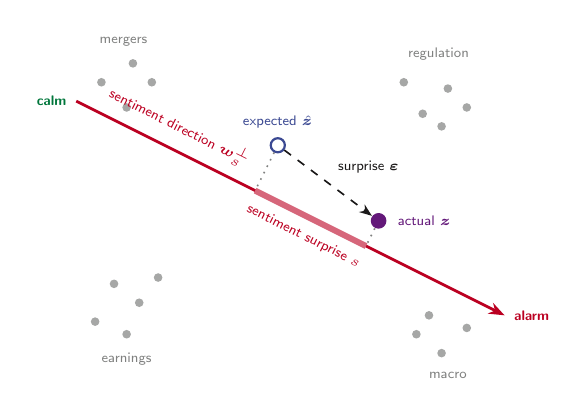
\begin{tikzpicture}[scale=0.8, dot/.style={circle, fill=sGray!70, inner sep=1.1pt}]
\foreach \p in {(-2.6,-1.3),(-2.2,-1.6),(-2.9,-1.9),(-2.4,-2.1),(-1.9,-1.2)} \node[dot] at \p {};
\node[lbl, text=sGray, font=\sffamily\tiny] at (-2.4,-2.5) {earnings};
\foreach \p in {(-2.4,1.5),(-2.0,1.9),(-2.8,1.9),(-2.3,2.2)} \node[dot] at \p {};
\node[lbl, text=sGray, font=\sffamily\tiny] at (-2.45,2.55) {mergers};
\foreach \p in {(2.3,1.4),(2.7,1.8),(2.0,1.9),(2.6,1.2),(3.0,1.5)} \node[dot] at \p {};
\node[lbl, text=sGray, font=\sffamily\tiny] at (2.55,2.35) {regulation};
\foreach \p in {(2.2,-2.1),(2.6,-2.4),(3.0,-2.0),(2.4,-1.8)} \node[dot] at \p {};
\node[lbl, text=sGray, font=\sffamily\tiny] at (2.7,-2.75) {macro};
\draw[-{Stealth[length=2mm]}, echo, line width=1.0pt] (-3.2,1.6) -- (3.6,-1.8);
\node[lbl, text=echo, anchor=west, font=\sffamily\tiny\bfseries] at (3.6,-1.8) {alarm};
\node[lbl, text=good!85!black, anchor=east, font=\sffamily\tiny\bfseries] at (-3.2,1.6) {calm};
\node[lbl, text=echo, rotate=-26.6, anchor=south, font=\sffamily\tiny] at (-1.7,0.9) {sentiment direction $\w_s^\perp$};
\node[circle, draw=do, line width=0.8pt, fill=white, inner sep=1.8pt] (ez) at (0,0.9) {};
\node[circle, fill=say, inner sep=2pt] (az) at (1.6,-0.3) {};
\node[lbl, text=do, anchor=south, font=\sffamily\tiny] at (0,1.02) {expected $\hat{\z}$};
\node[lbl, text=say, anchor=west, font=\sffamily\tiny] at (1.75,-0.3) {actual $\z$};
\draw[-{Stealth[length=1.6mm]}, dashed, ink, line width=0.6pt] (ez) -- (az) node[midway, above right, lbl, font=\sffamily\tiny] {surprise $\bm\varepsilon$};
\draw[dotted, sGray, line width=0.6pt] (ez) -- (-0.36,0.18);
\draw[dotted, sGray, line width=0.6pt] (az) -- (1.40,-0.70);
\draw[line width=2.2pt, echo!60] (-0.36,0.18) -- (1.40,-0.70);
\node[lbl, text=echo, rotate=-26.6, anchor=north, font=\sffamily\tiny] at (0.52,-0.32) {sentiment surprise $s$};
\end{tikzpicture}
\end{minipage}\hfill
\begin{minipage}[t]{0.5\textwidth}
\panel{b}
\centering
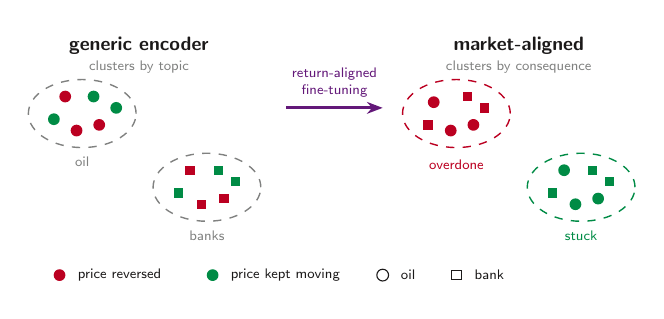
\begin{tikzpicture}[scale=0.72,
  cr/.style={circle, fill=echo, inner sep=1.5pt},
  cg/.style={circle, fill=good, inner sep=1.5pt},
  sr/.style={rectangle, fill=echo, inner sep=1.7pt},
  sg/.style={rectangle, fill=good, inner sep=1.7pt}]
\node[lbl, font=\sffamily\scriptsize\bfseries] at (2.3,3.4) {generic encoder};
\node[lbl, text=sGray, font=\sffamily\tiny] at (2.3,3.02) {clusters by topic};
\draw[dashed, sGray, line width=0.5pt] (1.3,2.2) ellipse (0.95 and 0.6);
\draw[dashed, sGray, line width=0.5pt] (3.5,0.9) ellipse (0.95 and 0.6);
\node[lbl, text=sGray, font=\sffamily\tiny] at (1.3,1.35) {oil};
\node[lbl, text=sGray, font=\sffamily\tiny] at (3.5,0.05) {banks};
\foreach \p in {(1.0,2.5),(1.6,2.0),(1.2,1.9)} \node[cr] at \p {};
\foreach \p in {(1.5,2.5),(0.8,2.1),(1.9,2.3)} \node[cg] at \p {};
\foreach \p in {(3.2,1.2),(3.8,0.7),(3.4,0.6)} \node[sr] at \p {};
\foreach \p in {(3.7,1.2),(3.0,0.8),(4.0,1.0)} \node[sg] at \p {};
\draw[-{Stealth[length=2mm]}, say, line width=1.0pt] (4.9,2.3) -- (6.6,2.3) node[midway, above, lbl, text=say, font=\sffamily\tiny, align=center] {return-aligned\\ fine-tuning};
\node[lbl, font=\sffamily\scriptsize\bfseries] at (9.0,3.4) {market-aligned};
\node[lbl, text=sGray, font=\sffamily\tiny] at (9.0,3.02) {clusters by consequence};
\draw[dashed, echo, line width=0.5pt] (7.9,2.2) ellipse (0.95 and 0.6);
\draw[dashed, good, line width=0.5pt] (10.1,0.9) ellipse (0.95 and 0.6);
\node[lbl, text=echo, font=\sffamily\tiny, anchor=north] at (7.9,1.55) {overdone};
\node[lbl, text=good, font=\sffamily\tiny] at (10.1,0.05) {stuck};
\foreach \p in {(7.5,2.4),(8.2,2.0),(7.8,1.9)} \node[cr] at \p {};
\foreach \p in {(8.1,2.5),(7.4,2.0),(8.4,2.3)} \node[sr] at \p {};
\foreach \p in {(9.8,1.2),(10.4,0.7),(10.0,0.6)} \node[cg] at \p {};
\foreach \p in {(10.3,1.2),(9.6,0.8),(10.6,1.0)} \node[sg] at \p {};
\node[cr] at (0.9,-0.65) {}; \node[lbl, anchor=west, font=\sffamily\tiny] at (1.05,-0.65) {price reversed};
\node[cg] at (3.6,-0.65) {}; \node[lbl, anchor=west, font=\sffamily\tiny] at (3.75,-0.65) {price kept moving};
\node[circle, draw=ink, inner sep=1.5pt] at (6.6,-0.65) {}; \node[lbl, anchor=west, font=\sffamily\tiny] at (6.75,-0.65) {oil};
\node[rectangle, draw=ink, inner sep=1.7pt] at (7.9,-0.65) {}; \node[lbl, anchor=west, font=\sffamily\tiny] at (8.05,-0.65) {bank};
\end{tikzpicture}
\end{minipage}
\caption{\textbf{A map of meaning aligned with markets.} \textbf{a},~Embeddings cluster by topic, sentiment is a direction, and surprise is measured against the \emph{expected} story; its projection onto the alarm direction is the sentiment surprise. \textbf{b},~At the optimum of the return-aligned objective (\cref{thm:racl}), distances mirror market aftermaths, so ``news that got overdone'' becomes a region of the map.}
\label{fig:embed}
\end{figure*}

\subsection{Who moved first? L\'evy area}\label{sec:leadlag}

For paths $X,Y$, the L\'evy area $\mathcal{A}_T=\tfrac12\int_0^T(X_u-X_0)\,dY_u-(Y_u-Y_0)\,dX_u$ is the antisymmetric part of the level-two signature. For a closed loop it is the signed enclosed area.

\begin{theorem}[Expected area identifies lead--lag]\label{thm:levy}
Let $(X,Y)$ be zero-mean, jointly stationary and mean-square $C^1$, with cross-covariance $C(h)=\E[X_sY_{s+h}]\in C^1$. Then
\[
  \E[\mathcal{A}_T]=T\,C'(0)-\tfrac12\big(C(T)-C(-T)\big),
\]
so $\E[\mathcal{A}_T]/T\to C'(0)$ when $C$ is bounded. If $Y_t=\gamma X_{t-\ell}+Z_t$, with $Z$ independent and $X$ having a unimodal autocovariance, then the limiting rate has the sign of $\gamma\ell$.
\end{theorem}

With $X$ = positioning and $Y$ = headline gloom, a positive area rate means that money moved first and the story turned against it (\cref{fig:loop}).

\begin{figure}[t]
\centering
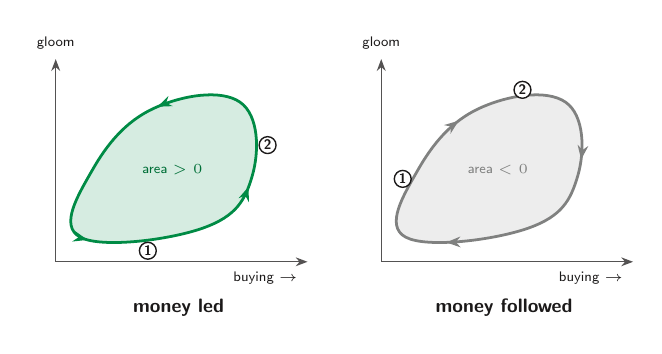
\begin{tikzpicture}[scale=0.78,
  arrowmid/.style={postaction={decorate}, decoration={markings,
    mark=at position 0.12 with {\arrow{Stealth[length=1.8mm]}},
    mark=at position 0.45 with {\arrow{Stealth[length=1.8mm]}},
    mark=at position 0.78 with {\arrow{Stealth[length=1.8mm]}}}}]
\begin{scope}
\draw[-{Stealth[length=1.5mm]}, ink!75, line width=0.5pt] (0,0) -- (4.1,0) node[below left, lbl, font=\sffamily\tiny] {buying $\rightarrow$};
\draw[-{Stealth[length=1.5mm]}, ink!75, line width=0.5pt] (0,0) -- (0,3.3) node[above, lbl, font=\sffamily\tiny] {gloom};
\fill[good!16] plot[smooth cycle, tension=0.7] coordinates {(0.4,0.4) (2.4,0.55) (3.2,1.4) (3.0,2.6) (1.6,2.5) (0.6,1.5)};
\draw[good, line width=1.0pt, arrowmid] plot[smooth cycle, tension=0.7] coordinates {(0.4,0.4) (2.4,0.55) (3.2,1.4) (3.0,2.6) (1.6,2.5) (0.6,1.5)};
\node[lbl, text=good!80!black, font=\sffamily\tiny] at (1.9,1.5) {area $>0$};
\node[numb] at (1.5,0.18) {1}; \node[numb] at (3.45,1.9) {2};
\node[lbl, font=\sffamily\scriptsize\bfseries, align=center] at (2.0,-0.75) {money led};
\end{scope}
\begin{scope}[xshift=5.3cm]
\draw[-{Stealth[length=1.5mm]}, ink!75, line width=0.5pt] (0,0) -- (4.1,0) node[below left, lbl, font=\sffamily\tiny] {buying $\rightarrow$};
\draw[-{Stealth[length=1.5mm]}, ink!75, line width=0.5pt] (0,0) -- (0,3.3) node[above, lbl, font=\sffamily\tiny] {gloom};
\fill[ink!8] plot[smooth cycle, tension=0.7] coordinates {(0.4,0.4) (0.6,1.5) (1.6,2.5) (3.0,2.6) (3.2,1.4) (2.4,0.55)};
\draw[sGray, line width=1.0pt, arrowmid] plot[smooth cycle, tension=0.7] coordinates {(0.4,0.4) (0.6,1.5) (1.6,2.5) (3.0,2.6) (3.2,1.4) (2.4,0.55)};
\node[lbl, text=sGray, font=\sffamily\tiny] at (1.9,1.5) {area $<0$};
\node[numb] at (0.35,1.35) {1}; \node[numb] at (2.3,2.8) {2};
\node[lbl, font=\sffamily\scriptsize\bfseries, align=center] at (2.0,-0.75) {money followed};
\end{scope}
\end{tikzpicture}
\caption{\textbf{Lead--lag as a loop.} Traced in the (positioning, gloom) plane, the orientation of the path shows who moved first, and its enclosed area shows how strongly (\cref{thm:levy}).}
\label{fig:loop}
\end{figure}

% =====================================================================
\section{From Signals to Decisions}\label{sec:decisions}

Events belong to latent regimes (informational, overreaction, strategic) with emissions $\bm o_t=(s^{\mathrm{new}},s^{\mathrm{echo}},G,A,\mathcal{A},\dots)$. Filtered regime probabilities are causal, and the MSE-optimal forecast is the mixture of regime experts. Strategic episodes of $n$ events are detected with error at most $\tfrac12e^{-n\Delta^2/8}$. Adaptive conformal intervals attain long-run coverage deterministically \citep{gibbs2021}. Positions use the shrunk Kelly fraction $c^\star=\mathrm{SNR}/(1+\mathrm{SNR})$, since full Kelly destroys growth when the edge is noisier than it is large (\cref{app:extra}). A transparent composite whose every sign is fixed by a theorem is
\begin{multline*}
  D=\omega_1s^{\mathrm{new}}-\omega_2s^{\mathrm{echo}}+\omega_3\,\mathrm{Do}\\
  +\widehat{\sgn}\,\omega_4\gamma\,\mathrm{Say}+\omega_5A+\omega_6\mathcal{A}^{\pm}.
\end{multline*}
Here $\widehat{\sgn}$ is the rolling sign of $\Cov(\text{Say},\text{Do})$ (\cref{thm:identity}): deeds are always followed, and words are followed when the covariance is positive and faded when it is negative, in which case the two terms combine into $-G_\gamma$ (\cref{thm:saydo}). $\mathcal{A}^\pm$ is the L\'evy area signed by the direction of positioning. \Cref{fig:pipeline} shows the complete architecture.

\begin{figure}[t]
\centering
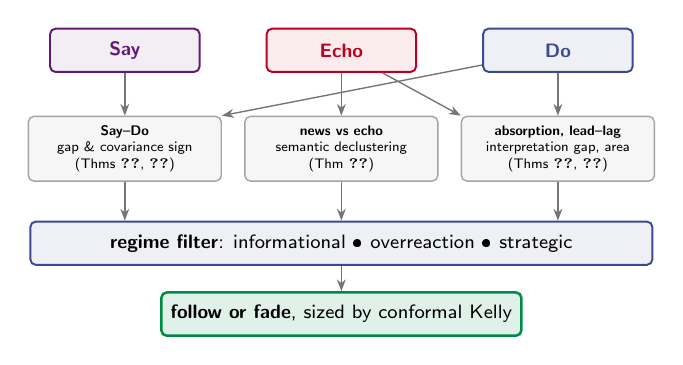
\begin{tikzpicture}[
  voice/.style={rounded corners=2pt, line width=0.7pt, minimum width=1.9cm, minimum height=0.55cm, align=center, font=\sffamily\scriptsize\bfseries},
  sig/.style={rounded corners=2pt, draw=ink!40, fill=ink!4, line width=0.5pt, minimum width=2.45cm, minimum height=0.78cm, align=center, font=\sffamily\tiny},
  arr/.style={-{Stealth[length=1.5mm]}, line width=0.5pt, ink!60}]
\node[voice, draw=say, fill=say!8, text=say] (say) at (0,0) {Say};
\node[voice, draw=echo, fill=echo!8, text=echo] (echo) at (2.75,0) {Echo};
\node[voice, draw=do, fill=do!8, text=do] (do) at (5.5,0) {Do};
\node[sig] (gap) at (0,-1.25) {\textbf{Say--Do}\\ gap \& covariance sign\\ (Thms~\ref{thm:saydo}, \ref{thm:identity})};
\node[sig] (news) at (2.75,-1.25) {\textbf{news vs echo}\\ semantic declustering\\ (Thm~\ref{thm:semantic})};
\node[sig] (abs) at (5.5,-1.25) {\textbf{absorption, lead--lag}\\ interpretation gap, area\\ (Thms~\ref{thm:absorption}, \ref{thm:levy})};
\node[rounded corners=2pt, draw=do, fill=do!8, line width=0.7pt, minimum width=7.9cm, minimum height=0.55cm, font=\sffamily\scriptsize, align=center] (reg) at (2.75,-2.45) {\textbf{regime filter}: informational \textbullet\ overreaction \textbullet\ strategic};
\node[rounded corners=2pt, draw=good, fill=good!12, line width=0.9pt, minimum width=4.2cm, minimum height=0.55cm, font=\sffamily\scriptsize, align=center] (dec) at (2.75,-3.35) {\textbf{follow or fade}, sized by conformal Kelly};
\draw[arr] (say) -- (gap); \draw[arr] (do) -- (gap.north east);
\draw[arr] (echo) -- (news); \draw[arr] (echo) -- (abs.north west); \draw[arr] (do) -- (abs);
\draw[arr] (gap) -- (gap|-reg.north); \draw[arr] (news) -- (news|-reg.north); \draw[arr] (abs) -- (abs|-reg.north);
\draw[arr] (reg) -- (dec);
\end{tikzpicture}
\caption{\textbf{Architecture.} Three voices produce three families of theorem-signed signals, and a regime filter turns them into a single calibrated decision.}
\label{fig:pipeline}
\end{figure}

% =====================================================================
\section{Numerical Verification}\label{sec:verify}

Every closed form was checked independently (\cref{tab:verify}). Gaussian results were checked by regression on $2\times10^6$ simulated draws. \Cref{thm:identity} was checked with fat-tailed values ($t_3$) and Laplace noise, which tests its distribution-free claim. The optimal speech of \cref{thm:speech} was checked against numerical optimisation. \Cref{thm:semantic} was checked by brute-force enumeration of all parent labellings, and \cref{thm:levy} on a smooth Gaussian process with a known lag.

\begin{table}[t]
\centering
\caption{\textbf{Theory versus simulation.} Theory values are exact; simulations use $2\times10^6$ draws (seed 0).}
\label{tab:verify}
\footnotesize
\setlength{\tabcolsep}{3.5pt}
\begin{tabularx}{\columnwidth}{@{}l>{\raggedright\arraybackslash}Xrr@{}}
\toprule
\textsf{Result} & \textsf{Quantity} & \textsf{Theory} & \textsf{Sim.} \\
\midrule
\cref{cor:echo} & Bayes weight on echo & $0$ & $-0.0006$ \\
\cref{thm:followfade} & loading, echo channel & $-0.1840$ & $-0.1843$ \\
\cref{thm:saydo} & loading on $\hat x$ ($c_x$) & $0.4012$ & $0.4004$ \\
\cref{thm:absorption} & absorption coefficient $c_A$ & $-0.1997$ & $-0.2004$ \\
\cref{thm:speech} & $(m^\ast,x^\ast)$, $\varphi{=}0.6$, $a{=}0.5$ & $(-0.714, 1.429)$ & $(-0.714, 1.429)$ \\
\cref{thm:identity} & $\Cov(r,\tilde m)$, $t_3$ values & $-2.294$ & $-2.293$ \\
\cref{thm:identity} & idem, exaggeration & $-7.608$ & $-7.676$ \\
\cref{thm:cycles} & 2-cycle at $a{=}1.95$ & $\{0.819, 1.131\}$ & $\{0.819, 1.131\}$ \\
\cref{thm:cycles} & multiplier, $a{=}1.8$ & $0$ & superstable \\
\cref{thm:semantic} & max posterior error & $0$ & $1.1{\times}10^{-16}$ \\
\cref{thm:levy} & area rate, lag $\ell=0.5$ & $0.2356$ & $0.2360$ \\
\cref{thm:kelly} & growth at $c^\star=0.338$ & $0.01056$ & $0.01055$ \\
\cref{thm:kelly} & growth at full Kelly & $-0.0300$ & $-0.0300$ \\
\bottomrule
\end{tabularx}
\end{table}

\begin{table}[t]
\centering
\caption{\textbf{Illustration: a hypothetical downgrade} (numbers are illustrative, not data).}
\label{tab:example}
\footnotesize
\begin{tabularx}{\columnwidth}{@{}Xr@{}}
\toprule
\textsf{Signal (result)} & \textsf{Reading} \\
\midrule
news / echo sentiment (Thm~\ref{thm:semantic}) & $-0.5\sigma$ / $-2.3\sigma$ \\
echo share $n$ (Prop.~\ref{prop:branching}) & $0.82$ \\
Say--Do covariance (Thm~\ref{thm:identity}) & negative: fade Say \\
implied vs actual move (Thm~\ref{thm:absorption}) & $-6.0\%$ vs $-1.9\%$ \\
L\'evy area rate (Thm~\ref{thm:levy}) & positive: money led \\
regime I / O / S & $0.10$ / $0.28$ / $0.62$ \\
Kelly fraction (Thm~\ref{thm:kelly}), SNR $\approx0.5$ & $c^\star\approx0.33$ \\
\midrule
\multicolumn{2}{@{}l@{}}{\textsf{\textbf{Reading:}} probable false alarm; lean long at one third of full Kelly.}\\
\bottomrule
\end{tabularx}
\end{table}

% =====================================================================
\section{Discussion}\label{sec:discussion}

\paragraph{Testable predictions} The theory predicts:
\begin{itemize}
  \item opposite signs on $s^{\mathrm{new}}$ and $s^{\mathrm{echo}}$;
  \item a negative Say--Do covariance in episodes later identified as manipulative;
  \item false alarms concentrated at intermediate echo shares in liquid markets, and exaggeration in illiquid ones;
  \item negative autocorrelation of the rolling Say--Do covariance where $\lambda k$ is moderate;
  \item an absorption loading whose sign flips with flow toxicity;
  \item higher returns after positive L\'evy area.
\end{itemize}
The cleanest first test pairs management tone on earnings calls (\SAY) with insider trades (\DO), both of which are public.

\paragraph{Limitations} Crowd pricing is reduced-form, and credulity is exogenous within a round. The price-formation results fix signs and sufficient statistics, not magnitudes. \Cref{thm:levy} assumes smooth, stationary paths. Empirical validation with point-in-time data and purged cross-validation \citep{lopezdeprado2018,bailey2014dsr} is left to companion work.

\paragraph{Ethics} A strategic reading means that narrative and capital moved in opposite directions in a particular order. It is not evidence of deception, and firms maintain information barriers between research and trading. The framework uses public information and lawful disclosures only. It must never be used to create or spread narratives intended to move prices.

% =====================================================================
{\small
\begin{thebibliography}{99}\setlength{\itemsep}{0pt}\footnotesize
\bibitem[Araci(2019)]{araci2019} D.~Araci. FinBERT: Financial sentiment analysis with pre-trained language models. arXiv:1908.10063, 2019.
\bibitem[Bacry et al.(2015)]{bacry2015} E.~Bacry, I.~Mastromatteo, J.-F.~Muzy. Hawkes processes in finance. \emph{Market Microstructure and Liquidity}, 1(1), 2015.
\bibitem[Bailey and L\'opez de Prado(2014)]{bailey2014dsr} D.~H.~Bailey, M.~L\'opez de Prado. The deflated Sharpe ratio. \emph{J.\ Portfolio Management}, 40(5):94--107, 2014.
\bibitem[Baker and Wurgler(2006)]{baker2006} M.~Baker, J.~Wurgler. Investor sentiment and the cross-section of stock returns. \emph{J.\ Finance}, 61(4):1645--1680, 2006.
\bibitem[Barber and Odean(2008)]{barber2008} B.~M.~Barber, T.~Odean. All that glitters: The effect of attention and news on the buying behavior of individual and institutional investors. \emph{Rev.\ Financial Studies}, 21(2):785--818, 2008.
\bibitem[B\'enabou and Laroque(1992)]{benabou1992} R.~B\'enabou, G.~Laroque. Using privileged information to manipulate markets: Insiders, gurus, and credibility. \emph{Quarterly J.\ Economics}, 107(3):921--958, 1992.
\bibitem[Bhattacharyya(1943)]{bhattacharyya1943} A.~Bhattacharyya. On a measure of divergence between two statistical populations. \emph{Bull.\ Calcutta Math.\ Soc.}, 35:99--109, 1943.
\bibitem[Bouchaud et al.(2018)]{bouchaud2018} J.-P.~Bouchaud, J.~Bonart, J.~Donier, M.~Gould. \emph{Trades, Quotes and Prices}. Cambridge University Press, 2018.
\bibitem[Brunnermeier and Pedersen(2005)]{brunnermeier2005} M.~K.~Brunnermeier, L.~H.~Pedersen. Predatory trading. \emph{J.\ Finance}, 60(4):1825--1863, 2005.
\bibitem[Chan(2003)]{chan2003} W.~S.~Chan. Stock price reaction to news and no-news: Drift and reversal after headlines. \emph{J.\ Financial Economics}, 70(2):223--260, 2003.
\bibitem[Chevyrev and Kormilitzin(2016)]{chevyrev2016} I.~Chevyrev, A.~Kormilitzin. A primer on the signature method in machine learning. arXiv:1603.03788, 2016.
\bibitem[Cohen et al.(2012)]{cohen2012} L.~Cohen, C.~Malloy, L.~Pomorski. Decoding inside information. \emph{J.\ Finance}, 67(3):1009--1043, 2012.
\bibitem[Crawford and Sobel(1982)]{crawford1982} V.~P.~Crawford, J.~Sobel. Strategic information transmission. \emph{Econometrica}, 50(6):1431--1451, 1982.
\bibitem[Da et al.(2011)]{da2011} Z.~Da, J.~Engelberg, P.~Gao. In search of attention. \emph{J.\ Finance}, 66(5):1461--1499, 2011.
\bibitem[De Long et al.(1990)]{delong1990} J.~B.~De Long, A.~Shleifer, L.~H.~Summers, R.~J.~Waldmann. Noise trader risk in financial markets. \emph{J.\ Political Economy}, 98(4):703--738, 1990.
\bibitem[Engelberg et al.(2012)]{engelberg2012} J.~E.~Engelberg, A.~V.~Reed, M.~C.~Ringgenberg. How are shorts informed? \emph{J.\ Financial Economics}, 105(2):260--278, 2012.
\bibitem[Evans and Honkapohja(2001)]{evans2001} G.~W.~Evans, S.~Honkapohja. \emph{Learning and Expectations in Macroeconomics}. Princeton University Press, 2001.
\bibitem[Ezekiel(1938)]{ezekiel1938} M.~Ezekiel. The cobweb theorem. \emph{Quarterly J.\ Economics}, 52(2):255--280, 1938.
\bibitem[Gibbs and Cand\`es(2021)]{gibbs2021} I.~Gibbs, E.~Cand\`es. Adaptive conformal inference under distribution shift. \emph{NeurIPS}, 34, 2021.
\bibitem[Glasserman and Lin(2023)]{glasserman2023} P.~Glasserman, C.~Lin. Assessing look-ahead bias in stock return predictions generated by GPT sentiment analysis. arXiv:2309.17322, 2023.
\bibitem[Glosten and Milgrom(1985)]{glosten1985} L.~R.~Glosten, P.~R.~Milgrom. Bid, ask and transaction prices in a specialist market with heterogeneously informed traders. \emph{J.\ Financial Economics}, 14(1):71--100, 1985.
\bibitem[Hawkes(1971)]{hawkes1971} A.~G.~Hawkes. Spectra of some self-exciting and mutually exciting point processes. \emph{Biometrika}, 58(1):83--90, 1971.
\bibitem[Hawkes and Oakes(1974)]{hawkesoakes1974} A.~G.~Hawkes, D.~Oakes. A cluster process representation of a self-exciting process. \emph{J.\ Applied Probability}, 11(3):493--503, 1974.
\bibitem[Hong and Stein(1999)]{hong1999} H.~Hong, J.~C.~Stein. A unified theory of underreaction, momentum trading, and overreaction in asset markets. \emph{J.\ Finance}, 54(6):2143--2184, 1999.
\bibitem[Kailath(1967)]{kailath1967} T.~Kailath. The divergence and Bhattacharyya distance measures in signal selection. \emph{IEEE Trans.\ Communication Technology}, 15(1):52--60, 1967.
\bibitem[Kartik et al.(2007)]{kartik2007} N.~Kartik, M.~Ottaviani, F.~Squintani. Credulity, lies, and costly talk. \emph{J.\ Economic Theory}, 134(1):93--116, 2007.
\bibitem[Ke et al.(2019)]{ke2019} Z.~T.~Ke, B.~T.~Kelly, D.~Xiu. Predicting returns with text data. NBER Working Paper 26186, 2019.
\bibitem[Kelly(1956)]{kelly1956} J.~L.~Kelly. A new interpretation of information rate. \emph{Bell System Technical J.}, 35(4):917--926, 1956.
\bibitem[Kogan et al.(2023)]{kogan2023} S.~Kogan, T.~J.~Moskowitz, M.~Niessner. Social media and financial news manipulation. \emph{Review of Finance}, 27(4):1229--1268, 2023.
\bibitem[Kyle(1985)]{kyle1985} A.~S.~Kyle. Continuous auctions and insider trading. \emph{Econometrica}, 53(6):1315--1335, 1985.
\bibitem[L\'evy(1940)]{levy1940} P.~L\'evy. Le mouvement brownien plan. \emph{American J.\ Mathematics}, 62(1):487--550, 1940.
\bibitem[Llorente et al.(2002)]{llorente2002} G.~Llorente, R.~Michaely, G.~Saar, J.~Wang. Dynamic volume-return relation of individual stocks. \emph{Rev.\ Financial Studies}, 15(4):1005--1047, 2002.
\bibitem[L\'opez de Prado(2018)]{lopezdeprado2018} M.~L\'opez de Prado. \emph{Advances in Financial Machine Learning}. Wiley, 2018.
\bibitem[Lopez-Lira and Tang(2023)]{lopezlira2023} A.~Lopez-Lira, Y.~Tang. Can ChatGPT forecast stock price movements? Return predictability and large language models. arXiv:2304.07619, 2023.
\bibitem[Loughran and McDonald(2011)]{loughran2011} T.~Loughran, B.~McDonald. When is a liability not a liability? Textual analysis, dictionaries, and 10-Ks. \emph{J.\ Finance}, 66(1):35--65, 2011.
\bibitem[Lyons(1998)]{lyons1998} T.~J.~Lyons. Differential equations driven by rough signals. \emph{Rev.\ Mat.\ Iberoamericana}, 14(2):215--310, 1998.
\bibitem[May(1976)]{may1976} R.~M.~May. Simple mathematical models with very complicated dynamics. \emph{Nature}, 261:459--467, 1976.
\bibitem[Merton(1969)]{merton1969} R.~C.~Merton. Lifetime portfolio selection under uncertainty: The continuous-time case. \emph{Rev.\ Economics and Statistics}, 51(3):247--257, 1969.
\bibitem[van den Oord et al.(2018)]{oord2018} A.~van den Oord, Y.~Li, O.~Vinyals. Representation learning with contrastive predictive coding. arXiv:1807.03748, 2018.
\bibitem[Park et al.(2023)]{park2023} K.~Park, Y.~J.~Choe, V.~Veitch. The linear representation hypothesis and the geometry of large language models. arXiv:2311.03658, 2023.
\bibitem[Reimers and Gurevych(2019)]{reimers2019} N.~Reimers, I.~Gurevych. Sentence-BERT: Sentence embeddings using Siamese BERT-networks. \emph{EMNLP-IJCNLP}, 2019.
\bibitem[Shleifer and Vishny(1997)]{shleifer1997} A.~Shleifer, R.~W.~Vishny. The limits of arbitrage. \emph{J.\ Finance}, 52(1):35--55, 1997.
\bibitem[Tetlock(2007)]{tetlock2007} P.~C.~Tetlock. Giving content to investor sentiment: The role of media in the stock market. \emph{J.\ Finance}, 62(3):1139--1168, 2007.
\bibitem[van Bommel(2003)]{vanbommel2003} J.~van Bommel. Rumors. \emph{J.\ Finance}, 58(4):1499--1520, 2003.
\bibitem[Veronesi(1999)]{veronesi1999} P.~Veronesi. Stock market overreaction to bad news in good times: A rational expectations equilibrium model. \emph{Rev.\ Financial Studies}, 12(5):975--1007, 1999.
\bibitem[Zhuang et al.(2002)]{zhuang2002} J.~Zhuang, Y.~Ogata, D.~Vere-Jones. Stochastic declustering of space-time earthquake occurrences. \emph{J.\ American Statistical Association}, 97(458):369--380, 2002.
\end{thebibliography}
}

% =====================================================================
\onecolumn
\appendix
\section{Proofs}\label{app:proofs}

\begin{lemma}[Gaussian conditioning]\label{lem:gauss}
If $(\bm a,\bm b)$ is jointly Gaussian with $\Var\bm b\succ0$, then $\E[\bm a\mid\bm b]=\E\bm a+\Cov(\bm a,\bm b)\Var(\bm b)^{-1}(\bm b-\E\bm b)$ and $\Var(\bm a\mid\bm b)=\Var\bm a-\Cov(\bm a,\bm b)\Var(\bm b)^{-1}\Cov(\bm b,\bm a)$. The same holds conditionally on a further jointly Gaussian vector.
\end{lemma}
\begin{proof}
The residual $\bm e=\bm a-\E\bm a-\Cov(\bm a,\bm b)\Var(\bm b)^{-1}(\bm b-\E\bm b)$ is uncorrelated with $\bm b$, and therefore independent of it by joint Gaussianity. Its variance expands to the stated formula.
\end{proof}

\paragraph{Price and return} From $x=\beta(v-p)$, $p(1+\lambda\beta)=\bphi^\top\y+\lambda\beta v+\lambda u$, so $r=v-p=\kappa(v-\bphi^\top\y-\lambda u)$.

\begin{proof}[Proof of \cref{thm:followfade}]
$\E[v\mid\y]=\sigma_v^2\h^\top\Sigma_y^{-1}\y=\w^{\star\top}\y$ and $\E[u\mid\y]=0$. The residual $r-\E[r\mid\y]=\kappa\big((v-\E[v\mid\y])-\lambda u\big)$ has independent components given $\y$.
\end{proof}

\begin{proof}[Proof of \cref{cor:echo}]
$\sigma(\y)=\sigma(\y_{-e},\xi)$ with $\xi$ independent of $(v,\y_{-e})$, so $\E[v\mid\y]=\E[v\mid\y_{-e}]$, which is linear in $\y_{-e}$ alone. If $\w^{\star\top}\y=\w'^\top\y$ almost surely with $w'_e=0$, then $(\w^\star-\w')^\top\Sigma_y(\w^\star-\w')=0$, and $\Sigma_y\succ0$ gives $\w^\star=\w'$.
\end{proof}

\begin{proof}[Proof of \cref{cor:news}]
Conditionally on $\y_{-n}$, $v\sim\N(\mu',s^2)$ with $s^2>0$. The scalar update puts weight $s^2/(s^2+\sigma_n^2)\in(0,1)$ on $n$. Apply \cref{thm:followfade}.
\end{proof}

\begin{proof}[Proof of \cref{thm:saydo}]
$x=\beta r$, so $\hat x=\beta r+\xi_x$. Given $\y$, $\Cov(r,\hat x)=\beta\varsigma^2$ and $\Var\hat x=\beta^2\varsigma^2+\sigma_x^2$. \Cref{lem:gauss} gives $\E[r\mid\y,\hat x]=(1-\beta c_x)\E[r\mid\y]+c_x\hat x$ with $1-\beta c_x=\theta$, and $\Var=\varsigma^2-c_x\beta\varsigma^2=\theta\varsigma^2$. The $(m,\hat x)$ terms are $-\theta\kappa(\varphi_1-w^\star_1)m+c_x\hat x=-c_x(\gamma m-\hat x)$.
\end{proof}

\begin{proof}[Proof of \cref{thm:absorption}]
Let $\tilde v=v-\E[v\mid\y]$. Then $r-\E[r\mid\y]=\kappa(\tilde v-\lambda u)$. Since $a=\lambda\beta r+\lambda u$, we get $a-\E[a\mid\y]=\lambda\beta\kappa\tilde v+\lambda(1-\lambda\beta\kappa)u=\lambda\kappa(\beta\tilde v+u)$, using $1-\lambda\beta\kappa=\kappa$. Hence $\Cov(r,a\mid\y)=\lambda\kappa^2(\beta\sigma^2_{v|y}-\lambda\sigma_u^2)$ and $\Var(a\mid\y)=\lambda^2\kappa^2(\beta^2\sigma^2_{v|y}+\sigma_u^2)$. Their ratio is $c_A$ by \cref{lem:gauss}. At Kyle's intensities, $\beta\sigma^2_{v|y}=\sigma_u\sigma_{v|y}$ and $\lambda\sigma_u^2=\tfrac12\sigma_u\sigma_{v|y}$, which give $c_A=\tfrac12$.
\end{proof}

\begin{proof}[Proof of \cref{lem:robust}]
$\hat a=a+(\bphi-\hat\bphi)^\top\y$ is an invertible affine map of $a$ given $\y$.
\end{proof}

\begin{proof}[Proof of \cref{thm:speech}]
$J$ is quadratic with Hessian $H=\begin{psmallmatrix}-2\lambda&-\varphi\\-\varphi&-k\end{psmallmatrix}$, which is negative definite iff $\det H=a-\varphi^2>0$. Then $J$ is strictly concave, and its unique maximiser solves $v-\varphi m-2\lambda x=0$ and $-\varphi x-k(m-v)=0$. Substitution gives $m(a-\varphi^2)=v(a-\varphi)$, and $1-\varphi\psi=a(1-\varphi)/(a-\varphi^2)$ gives $\chi$. If $\det H<0$, then $J(t\bm d)\to\infty$ along an eigenvector $\bm d$ with positive eigenvalue.
\end{proof}

\begin{proof}[Proof of \cref{cor:taxonomy}]
$\psi>0\iff a>\varphi$; $\psi<1\iff\varphi<1$; and $\sgn\chi=\sgn(1-\varphi)$. If $\varphi>1$, then $a>\varphi^2>\varphi$, so $\psi>1$.
\end{proof}

\begin{proof}[Proof of \cref{thm:identity}]
Given $m$, the optimal trade is $x=(v-\varphi m)/(2\lambda)$, so $v-\varphi m=2\lambda x$ and $r=v-\varphi(m+\varepsilon)-\lambda x=\lambda x-\varphi\varepsilon$. Since $x$ and $m$ are functions of $v$, which is independent of $\varepsilon$, we have $\Cov(\varepsilon,\tilde m)=\sigma_\varepsilon^2$ and $\E[\varepsilon\mid x]=0$. In equilibrium, $\Cov(\chi v,\psi v)=\psi\chi\sigma_v^2$, and $\psi\chi<0$ exactly in the false-alarm and exaggeration regimes.
\end{proof}

\begin{proof}[Proof of \cref{prop:virality}]
$\varphi=\varphi_0/(1-n)$ increases from $\varphi_0$ to $\infty$. A false alarm needs $\varphi^2<a<\varphi<1$, hence $a<1$. Exaggeration needs $1<\varphi<\sqrt a$, hence $a>1$. The conditions $\varphi>a$, $\varphi>1$ and $\varphi<\sqrt a$ translate to $n>1-\varphi_0/a$, $n>1-\varphi_0$ and $n<1-\varphi_0/\sqrt a$. For $a<1$, $\varphi<\sqrt a$ already implies $\varphi<1$.
\end{proof}

\begin{proof}[Proof of \cref{thm:cycles}]
(i) $F_a(\varphi)=\varphi\iff\varphi=1$, and admissibility ($\varphi^2<a$) needs $a>1$.
(ii) $F_a'(\varphi)=(a-2a\varphi+\varphi^2)/(a-\varphi)^2$, so $F_a'(1)=-1/(a-1)$, whose modulus is below $1$ iff $a>2$.
(iii) Using $a-F_a(\varphi)=(a^2-a\varphi-a+\varphi^2)/(a-\varphi)$, direct computation gives
\[
  F_a(F_a(\varphi))-\varphi=\frac{-a(\varphi-1)(2\varphi^2-2a\varphi+a^2-a)}{(a-\varphi)^2\big(a-F_a(\varphi)\big)} .
\]
The quadratic factor has roots $\varphi_\pm$, which are real and different from $1$ for $1<a<2$; its value at $\varphi=1$ is $(a-1)(a-2)\neq0$. They are admissible: $\varphi_\pm^2=\tfrac a2\big(1\pm\sqrt{a(2-a)}\big)<a$ because $a(2-a)<1$; $\varphi_\pm<a$ because $\sqrt{a(2-a)}<a\iff a>1$; and $\psi(\varphi_\pm)>0$. On the cycle, $\varphi^2=a\varphi-(a^2-a)/2$, so the numerator of $F'_a$ equals $a(3-a-2\varphi)/2$. With $\varphi_++\varphi_-=a$ and $\varphi_+\varphi_-=(a^2-a)/2$, we get $(3-a-2\varphi_+)(3-a-2\varphi_-)=(5a-9)(a-1)$ and $(a-\varphi_+)(a-\varphi_-)=a(a-1)/2$. Hence the multiplier is $(5a-9)/(a-1)$, whose modulus is below $1$ iff $\tfrac53<a<2$ when $1<a<2$.
(iv) At $a=2$ the multiplier is $1$ and $\varphi_\pm=1$; at $a=\tfrac53$ it is $-1$.
\end{proof}

\begin{proof}[Proof of \cref{prop:branching}]
Each news article founds a Galton--Watson cluster of expected size $\sum_kn^k=(1-n)^{-1}$. News arrives at rate $\mu$, so articles arrive at rate $\mu/(1-n)$, and the news share is $1-n$.
\end{proof}

\begin{proof}[Proof of \cref{thm:semantic}]
In the cluster representation, a labelled configuration is a realisation of independent Poisson streams: news at rate $\rho_0=\mu$, and echoes of $l$ at rate $\rho_l(t)=g(t-\tau_l)\ind\{t>\tau_l\}$. Its density is the product of the stream likelihoods and the mark densities,
\[
  e^{-\int_0^T\lambda}\prod_{j}\rho_{\pi(j)}(\tau_j)\,f_{\pi(j)}(\z_j),\qquad f_0\ \text{(news)},\quad f_l=f(\cdot\mid\z_l),
\]
because $\sum_k\rho_k=\lambda$. This factorises over $j$. Summing over labellings gives $e^{-\int\lambda}\prod_j\Lambda_j$, so the posterior is a product of the stated categorical laws. Because $s_j$ is a function of $\z_j$, $\E[\ind\{\pi(j)=0\}s_j\mid\cdot]=s_jp^{\mathrm{sem}}_j$. Integrating out the marks recovers the timing-only posterior, and conditioning does not increase expected entropy.
\end{proof}

\begin{proof}[Proof of \cref{thm:racl}]
Per anchor, $-\sum_kq_{jk}\log p_{jk}=H(q_{j\cdot})+\KL(q_{j\cdot}\|p_{j\cdot})$, with equality to $H(q_{j\cdot})$ iff $p_{j\cdot}=q_{j\cdot}$, that is, iff the logits differ by a constant $c_j$: $S_{jk}/\tau+D_{jk}/2b^2=c_j/\tau$. Symmetry of $S$ and $D$ forces $c_j=c_k$ for every pair, and on the sphere $\|\z_j-\z_k\|^2=2-2S_{jk}$.
\end{proof}

\begin{proof}[Proof of \cref{thm:robustnn}]
Pinsker gives $\sum_k|p_{jk}-q_{jk}|\le\sqrt{2\epsilon_j}$, so $p_{jk}-p_{jl}\ge q_{jk}-q_{jl}-\sqrt{2\epsilon_j}>0$. Softmax is monotone in $S_{j\cdot}$, so $S_{jk}>S_{jl}$, which gives the distance ordering.
\end{proof}

\begin{proof}[Proof of \cref{thm:levy}]
Mean-square differentiability gives $\E[X_s\dot Y_t]=C'(t-s)$ and $\E[Y_s\dot X_t]=-C'(s-t)$. Hence $\E[(X_u-X_0)\dot Y_u]=C'(0)-C'(u)$ and $\E[(Y_u-Y_0)\dot X_u]=-C'(0)+C'(-u)$. By Fubini,
\[
  \E[\mathcal{A}_T]=\tfrac12\int_0^T\big(2C'(0)-C'(u)-C'(-u)\big)\,du=TC'(0)-\tfrac12\big(C(T)-C(-T)\big).
\]
For $Y_t=\gamma X_{t-\ell}+Z_t$, $C(h)=\gamma R(h-\ell)$, so $C'(0)=-\gamma R'(\ell)$. This has the sign of $\gamma\ell$ when $R$ is even with $R'<0$ on $(0,\infty)$.
\end{proof}

\section{Additional Results}\label{app:extra}

\begin{proposition}[Causal filtering and mixture optimality]\label{prop:filter}
Filtered regime probabilities $\pi_t\propto f(\bm o_t)\odot P^\top\pi_{t-1}$ are $\F_t$-measurable, and $\E[r_{t+h}\mid\F_t]=\sum_k\pi_t(k)\E[r_{t+h}\mid\F_t,K_t=k]$. Smoothed probabilities are not $\F_t$-measurable in general and must not be used for forecasting.
\end{proposition}
\begin{proof}
The recursion is Bayes' rule, and the mixture follows from the tower property.
\end{proof}

\begin{theorem}[Exponential detectability]\label{thm:detect}
For $n$ events that are i.i.d.\ within a regime, with emissions $\N(\bm m_i,\Sigma)$ and priors $\pi_i$, the MAP error satisfies $P_e\le\sqrt{\pi_0\pi_1}\,e^{-n\Delta^2/8}\le\tfrac12e^{-n\Delta^2/8}$, where $\Delta^2=(\bm m_1-\bm m_0)^\top\Sigma^{-1}(\bm m_1-\bm m_0)$.
\end{theorem}
\begin{proof}
$\min\{a,b\}\le\sqrt{ab}$ gives $P_e\le\sqrt{\pi_0\pi_1}\,\mathrm{BC}^n$ \citep{bhattacharyya1943,kailath1967}. For equal-covariance Gaussians, completing the square gives $\mathrm{BC}=\int\sqrt{p_0p_1}=e^{-\Delta^2/8}$.
\end{proof}

\begin{theorem}[Adaptive conformal coverage; \citealp{gibbs2021}, Prop.~4.1]\label{thm:aci}
With nested sets $\hat C_t(\alpha')$ that equal $\R$ for $\alpha'\le0$ and $\emptyset$ for $\alpha'\ge1$, and the update $\alpha_{t+1}=\alpha_t+\gamma(\alpha-\mathrm{err}_t)$, every outcome sequence satisfies $|\frac1T\sum_t\mathrm{err}_t-\alpha|\le(\max\{\alpha_1,1-\alpha_1\}+\gamma)/(\gamma T)$.
\end{theorem}
\begin{proof}[Proof (reproduced)]
By induction, $\alpha_t\in[-\gamma,1+\gamma]$. Telescoping gives $\alpha_{T+1}-\alpha_1=\gamma\sum_t(\alpha-\mathrm{err}_t)$.
\end{proof}

\begin{theorem}[Kelly shrinkage under estimation risk; classical]\label{thm:kelly}
With excess growth rate $g(f)=f\mu-\tfrac12f^2\sigma^2$ \citep{merton1969,kelly1956}, an unbiased estimate $\hat\mu$ with variance $s^2$ that is independent of future returns, and $f=c\hat\mu/\sigma^2$, the expected growth is $\E g=(c\mu^2-\tfrac12c^2(\mu^2+s^2))/\sigma^2$. It is maximised at $c^\star=\mu^2/(\mu^2+s^2)$. Full Kelly yields $(\mu^2-s^2)/(2\sigma^2)$, which is negative when $s>|\mu|$.
\end{theorem}
\begin{proof}
Expand $\E[f\mu]$ and $\E[f^2]$ and maximise the resulting concave quadratic in $c$.
\end{proof}

\begin{proposition}[Analog forecasting]\label{prop:analog}
If $\mathrm{AR}_j=\mu(\z_j)+e_j$ with uncorrelated mean-zero errors of variance at most $\sigma^2$, $\mu$ is $L$-Lipschitz, and weights $\omega_j\ge0$ sum to one, then the estimator $\hat\mu(\z)=\sum_j\omega_j\mathrm{AR}_j$ has bias at most $L\sum_j\omega_jd(\z,\z_j)$ and variance at most $\sigma^2\sum_j\omega_j^2$.
\end{proposition}

\begin{proposition}[Calibrated surprise]\label{prop:surprise}
If $\z\mid\F\sim\N(\hat\z,\Sigma)$, then $S=(\z-\hat\z)^\top\Sigma^{-1}(\z-\hat\z)\sim\chi^2_D$, and $S$ equals Shannon surprisal up to additive constants.
\end{proposition}

\begin{figure}[h]
\centering
\begin{minipage}[t]{0.48\textwidth}
\panel{a}
\centering
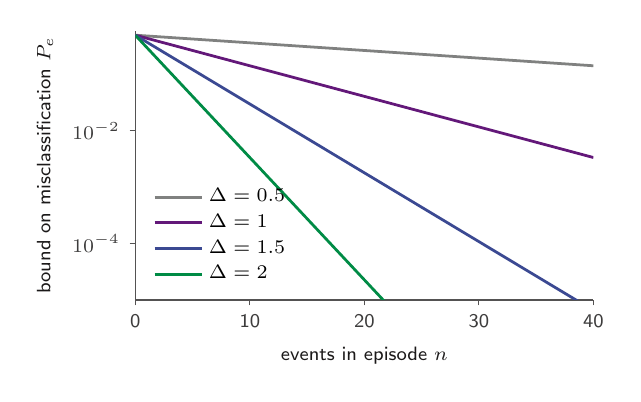
\begin{tikzpicture}
\begin{semilogyaxis}[sci, log basis y=10, yticklabel={$10^{\pgfmathprintnumber{\tick}}$}, width=7.4cm, height=5.0cm, xmin=0, xmax=40, ymin=1e-5, ymax=0.6,
  xlabel={events in episode $n$}, ylabel={bound on misclassification $P_e$},
  legend style={at={(0.02,0.02)}, anchor=south west}, samples=80, domain=0:40]
\addplot[sGray] {0.5*exp(-x*0.25/8)}; \addlegendentry{$\Delta=0.5$}
\addplot[say] {0.5*exp(-x*1/8)}; \addlegendentry{$\Delta=1$}
\addplot[do] {0.5*exp(-x*2.25/8)}; \addlegendentry{$\Delta=1.5$}
\addplot[good] {0.5*exp(-x*4/8)}; \addlegendentry{$\Delta=2$}
\end{semilogyaxis}
\end{tikzpicture}
\end{minipage}\hfill
\begin{minipage}[t]{0.48\textwidth}
\panel{b}
\centering
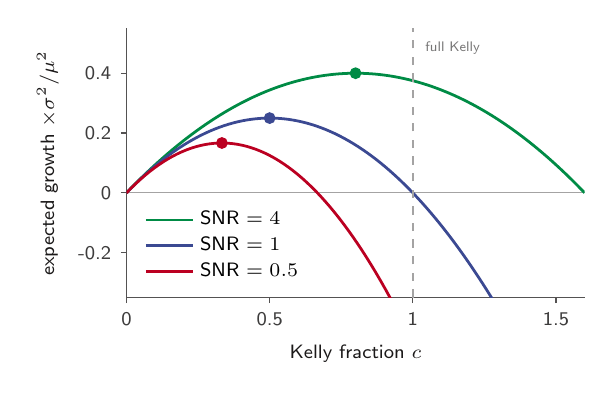
\begin{tikzpicture}
\begin{axis}[sci, width=7.4cm, height=5.0cm, xmin=0, xmax=1.6, ymin=-0.35, ymax=0.55,
  xlabel={Kelly fraction $c$}, ylabel={expected growth $\times\sigma^2/\mu^2$},
  legend style={at={(0.02,0.02)}, anchor=south west}, samples=100, domain=0:1.6]
\addplot[ink!40, line width=0.4pt, forget plot] coordinates {(0,0) (1.6,0)};
\addplot[good] {x - 0.5*x^2*(1+1/4)}; \addlegendentry{SNR $=4$}
\addplot[do] {x - 0.5*x^2*(1+1/1)}; \addlegendentry{SNR $=1$}
\addplot[echo] {x - 0.5*x^2*(1+1/0.5)}; \addlegendentry{SNR $=0.5$}
\addplot[only marks, mark=*, mark size=1.6pt, good, forget plot] coordinates {(0.8,0.4)};
\addplot[only marks, mark=*, mark size=1.6pt, do, forget plot] coordinates {(0.5,0.25)};
\addplot[only marks, mark=*, mark size=1.6pt, echo, forget plot] coordinates {(0.3333,0.16667)};
\addplot[ink!40, line width=0.5pt, dashed, forget plot] coordinates {(1,-0.35) (1,0.55)};
\node[lbl, text=ink!60, anchor=south west, font=\sffamily\tiny] at (axis cs:1.01,0.43) {full Kelly};
\end{axis}
\end{tikzpicture}
\end{minipage}
\caption{\textbf{Detection and sizing.} \textbf{a},~Misclassification of strategic episodes decays exponentially in episode length (\cref{thm:detect}). \textbf{b},~Expected growth as a function of the Kelly fraction; dots mark $c^\star=\mathrm{SNR}/(1+\mathrm{SNR})$ (\cref{thm:kelly}).}
\label{fig:sizing}
\end{figure}

\section{Implementation Notes}\label{app:impl}

\paragraph{Encoder} A transformer sentence encoder \citep{reimers2019} with low-rank adapters, trained on the return-aligned loss plus a KL anchor to the frozen encoder, on rolling windows whose outcome horizons close before each refit date. Pretrained components must predate each test window \citep{glasserman2023}.

\paragraph{Echo} Exponential Hawkes kernels are fitted per semantic cluster, with von Mises--Fisher echo marks. The posteriors of \cref{thm:semantic} cost $O(N\cdot\bar k)$ with $\bar k$ candidate parents retrieved from a vector index.

\paragraph{Say--Do} Pair management tone with insider trades, and published house views with disclosed holdings or futures positioning. A lag-augmented Kalman filter merges disclosures of mixed frequency, and a rolling window estimates $\Cov(\text{Say},\text{Do})$.

\paragraph{Validation} Point-in-time data, combinatorial purged cross-validation and deflated performance statistics \citep{lopezdeprado2018,bailey2014dsr}.

\end{document}
